\documentclass{beamer}

\usetheme[nophoto]{polimi}

% Full instructions available at:
% https://github.com/elauksap/beamerthemepolimi

% Set custom font (requires to compile with XeLaTeX).
\usepackage{ifxetex}
\ifxetex
    \usepackage{fontspec}
    \setsansfont[Scale=0.95]{Arial}
\fi

\usepackage{lipsum}

\title{Numerical Methods for partial differential Equations}
\subtitle{Cardiac electrophysiology}
\author{A. Reyes, C. Sciancalepore, A. Tomita, R. Zucchi}
\date{9 July 2026}

\begin{document}
    \begin{frame}
        \maketitle
        % If the theme option "nologo" is specified, a custom logo
        % can be added with the following commands:
        %\begin{tikzpicture}[overlay, remember picture]
        %    \node at (current page.north) [anchor=north, inner sep=2cm]
        %    {
        %        
\includegraphics[width=0.3\paperwidth]{logo_centrato_BN_negativo.png}
        %    };
        %\end{tikzpicture}
    \end{frame}


    
    
    % \section{Section 1}
    % % Section page.
    % \begin{frame}[plain]{}
    %     \sectionpage
    % \end{frame}
    
    % \begin{frame}{Slide 1}
    %     \lipsum[1]
    % \end{frame}
    
    % \subsection{Subsection 1.1}
    % \begin{frame}[plain]{}
    %     \subsectionpage
    % \end{frame}
    % \begin{frame}
    %     This frame has an empty title.
    %     \vfill
    %     \begin{itemize}
    %         \item item 1
    %         \begin{itemize}
    %             \item item 1.1
    %             \item item 1.2
    %         \end{itemize}
    %         \item item 2
    %         \item item 3
    %     \end{itemize}
    % \end{frame}
    
    % \subsection{Subsection 1.2}
    % % Slide without numbering.
    % \begin{frame}[nonumber]{Slide 1.2 without numbering}
    %     \lipsum[2]
    % \end{frame}
    
    % \section[Short]{Section 2}
    % \begin{frame}{Slide 2}
    %     \begin{block}{Block}
    %         Text.
    %     \end{block}
    %     \pause
    %     \begin{alertblock}{Alert block}
    %         Alert \alert{text}.
    %     \end{alertblock}
    %     \pause
    %     \begin{exampleblock}{Example block}
    %         Example \textcolor{greenPolimi}{text}.
    %     \end{exampleblock}
    % \end{frame}





\begin{frame}{Table of contents}
  \tableofcontents
\end{frame}









% ============================================================
\section{Introduction}
% ============================================================

\begin{frame}{Bueno-Orovio Minimal Ventricular Model}
\begin{itemize}
  \item Detailed ionic models (TNNP, IMW) incorporate dozens of variables via
        Hodgkin-Huxley equations or Markov chains.
  \item Two major limitations:
  \begin{itemize}
    \item computationally heavy $\Rightarrow$ 3D organ simulations impractical;
    \item high dimensionality obscures the link between a single parameter
          and macroscopic properties (APD,  action potential duration restitution).
  \end{itemize}
  \item \textbf{Minimal Ventricular (MV) model} (Bueno-Orovio, Cherry, Fenton, 2008):
        aggregates all transmembrane currents into three functional categories:
  \begin{enumerate}
    \item $J_{fi}$ -- fast inward current (upstroke);
    \item $J_{si}$ -- slow inward current (plateau);
    \item $J_{so}$ -- slow outward current (repolarization).
  \end{enumerate}
\end{itemize}
\end{frame}

% ============================================================
\section{Mathematical Formulation}
% ============================================================

\begin{frame}{Monodomain--Bueno-Orovio System}
\begin{equation*}
\left\{
\begin{array}{ll}
\displaystyle
\frac{\partial v}{\partial t}
-\boldsymbol{\nabla}\cdot(\Sigma\boldsymbol{\nabla} v)
+J_{\mathrm{ion}}(v,\mathbf{w})
=J_{\mathrm{app}}
& \text{in }\Omega, \\
\Sigma\boldsymbol{\nabla} v\cdot\mathbf{n} = 0
& \text{on }\partial\Omega, \\
v(t=0)=v_0
& \text{in }\Omega, \\
\displaystyle
\frac{d\mathbf{w}}{dt}=\mathbf{F}_{\mathrm{BO}}(v,\mathbf{w})
& \text{in }\Omega, \\
\mathbf{w}(t=0)=\mathbf{w}_0
& \text{in }\Omega.
\end{array}
\right.
\end{equation*}
\begin{itemize}
  \item $v$: dimensionless transmembrane potential ($0$=rest, $\approx 1$=peak)\\
  $V_{mV} = 85.7\,v - 84$ (conversion to physical units),
  \item $\mathbf{w} = (w_1,w_2,w_3)^T$: gating variables.
\end{itemize}
\end{frame}

\begin{frame}{Anisotropy Tensor}
The harmonic mean
\[
  \sigma_{\parallel} = \frac{\sigma_{i,\parallel}\,\sigma_{e,\parallel}}
  {\sigma_{i,\parallel}+\sigma_{e,\parallel}}, \qquad
  \sigma_{\perp} = \frac{\sigma_{i,\perp}\,\sigma_{e,\perp}}
  {\sigma_{i,\perp}+\sigma_{e,\perp}}
\]
where ($\sigma_{i,\parallel}, \sigma_{e,\parallel},
\sigma_{i,\perp}, \sigma_{e,\perp}$) are the intracellular and
extracellular longitudinal and transverse conductivities.
\[
  D_{\parallel} = \frac{\sigma_{\parallel}}{C_m\,\beta}, \qquad
  D_{\perp} = \frac{\sigma_{\perp}}{C_m\,\beta},
\]
\begin{itemize}
  \item $C_m$: the \textbf{membrane capacitance} (how much electric charge
        the cell membrane can store per unit surface area);
  \item $\beta$: the \textbf{surface-to-volume ratio} of the cells (how
        much membrane area is present per unit volume of tissue).
\end{itemize}
\begin{equation*}
\Sigma = \mathrm{diag}(D_{\parallel},
D_{\perp}, D_{\perp})
\end{equation*}
    
\end{frame}

\begin{frame}{Gating Variable Dynamics}
The model is governed by a system of four differential equations where $v$ is the transmembrane voltage and $\mathbf{w}=(w_1, w_2, w_3)^T$ is the vector of the three gating variables.
\begin{equation*}
    \frac{\partial v}{\partial t} = \boldsymbol{\nabla} \cdot \left( \Sigma\boldsymbol{\nabla} v \right) - \left( J_{fi} + J_{so} + J_{si} \right) + J_{app}
    \label{eq:placeholder_label}
\end{equation*}

\[
\frac{\partial w_1}{\partial t} = (1-H(v-\theta_{w1}))\frac{w_{1,\infty}-w_1}{\tau^-_{w1}}
 - H(v-\theta_{w1})\frac{w_1}{\tau^+_{w1}}
\]
\[
\frac{\partial w_2}{\partial t} = (1-H(v-\theta_{w2}))\frac{w_{2,\infty}-w_2}{\tau^-_{w2}}
 - H(v-\theta_{w2})\frac{w_2}{\tau^+_{w2}}
\]
\[
\frac{\partial w_3}{\partial t} = \frac{\dfrac{1+\tanh(k_{w3}(v-v_{w3}))}{2} - w_3}{\tau_{w3}}
\]
\end{frame}

\begin{frame}{Ionic Currents}
\[
J_{fi} = -w_1\cdot H(v-\theta_{w1})\cdot(v-\theta_{w1})\cdot\frac{(v_v-v)}{\tau_{fi}}
\]
\[
J_{so} = (v-v_o)\cdot\frac{1-H(v-\theta_{w2})}{\tau_o} + \frac{H(v-\theta_{w2})}{\tau_{so}}
\]
\[
J_{si} = -H(v-\theta_{w2})\cdot\frac{w_2\cdot w_3}{\tau_{si}}
\]
\begin{itemize}
  \item $J_{fi}$: phase-0 upstroke;
  \item $J_{so}$: repolarizing potassium current;
  \item $J_{si}$: L-type calcium current ($I_{CaL}$), sustains the plateau.
\end{itemize}
\end{frame}

% ============================================================
\section{Weak and Semi-Discrete Formulation}
% ============================================================

\begin{frame}{Weak Formulation}
Find $v(t)\in V=H^1(\Omega)$, $w(t)\in W=L^2(\Omega)$ such that $\forall\,\varphi\in V,\ \psi\in W$:
\[
\begin{cases}
\displaystyle\int_\Omega \frac{\partial v}{\partial t}\varphi
 + a(v,\varphi) + \int_\Omega J_{ion}(v,w)\,\varphi = \int_\Omega J_{app}\,\varphi, \\[8pt]
\displaystyle\int_\Omega \frac{\partial w}{\partial t}\psi = \int_\Omega F_{BO}(v,w)\,\psi,
\end{cases}
\]
with bilinear form
\[
a(u,\varphi) = \int_\Omega (\Sigma\nabla u)\cdot\nabla\varphi\,dx.
\]
\end{frame}

\begin{frame}{Semi-Discrete Problem}
Finite element spaces $V_h\subset V$, $W_h\subset W$:
\[
v_h(x,t) = \sum_{j=1}^{N} V_j(t)\varphi_j(x), \qquad
w_{k,h}(x,t) = \sum_{j=1}^{N_w} W_{k,j}(t)\psi_j(x),\ k=1,2,3.
\]
Resulting PDE-ODE system:
\[
\begin{cases}
M_v\dot V(t) + A_v V(t) + I_{ion}(V(t),W(t)) = I_{app}(t), \\
M_w \dot W(t) = F_{BO}(V(t),W(t)).
\end{cases}
\]
\[
(M_v)_{ij} = \int_\Omega \varphi_j\varphi_i\,dx,\qquad
(A_v)_{ij} = \int_\Omega (\Sigma\nabla\varphi_j)\cdot\nabla\varphi_i\,dx.
\]
\end{frame}

% ============================================================
\section{Time Discretization}
% ============================================================

\begin{frame}{Generalized $\theta$-Method (IMEX)}
\begin{itemize}
  \item Diffusion term: generalized $\theta$-method.
  \item Nonlinear ionic current: treated \textbf{explicitly}.
\end{itemize}
\[
V^{n+\theta} = (1-\theta)V^n + \theta V^{n+1}, \qquad 0\le\theta\le 1.
\]
Semi-discrete equation:
\[
M_v\frac{V^{n+1}-V^n}{\Delta t} + A_v V^{n+\theta} + I_{ion}(V^n,W^{n+1}) = I_{app}^{n+1}
\]
Expanding the intermediate value:
{\small
\[
\left(\frac{1}{\Delta t}M_v + \theta A_v\right)V^{n+1} =
\left(\frac{1}{\Delta t}M_v - (1-\theta)A_v\right)V^n - I_{ion}(V^n,W^{n+1}) + I_{app}^{n+1}
\]
}
\end{frame}

\begin{frame}{Crank-Nicolson Case ($\theta = 1/2$)}
\[
M_v\frac{V^{n+1}-V^n}{\Delta t} + A_v\left(\frac{V^{n+1}+V^n}{2}\right)
 + I_{ion}(V^n,W^{n+1}) = I_{app}^{n+1}
\]
\vspace{6pt}
Gating variables (explicit forward Euler):
\[
M_w\frac{W^{n+1}-W^n}{\Delta t} = F_{BO}(V^n,W^n)
\]
\begin{itemize}
  \item Decouples the ODE system (gating) from the PDE (diffusion);
  \item Gating variables updated \emph{before} assembling the RHS;
  \item Avoids solving a coupled nonlinear system at each time step.
\end{itemize}
\end{frame}

% ============================================================
\section{Fully Discrete Problem}
% ============================================================

\begin{frame}{Linear System for the Potential}
\[
K = \frac{1}{\Delta t}M_v + \theta A_v \quad %\text{(assembled once in \texttt{setup()})}
\]
\[
F^n = \frac{1}{\Delta t}M_vV^n - (1-\theta)A_vV^n - I_{ion}(V^n,W^{n+1}) + I_{app}^{n+1}
\]
\[
K\,V^{n+1} = F^n
\]
\begin{itemize}
  \item $K$ is time-independent $\Rightarrow$ assembled only once;
  \item $I_{ion}^n$ evaluated at the n-time level, \emph{not} averaged with $\theta$
        $\Rightarrow$ IMEX variant.
        % not a fully symmetric Crank-Nicolson.
\end{itemize}
\end{frame}

% \begin{frame}{Applied Stimulus Current $I_{app}$}
% \[
% I_{app}(x,t) =
% \begin{cases}
% I_0, & x\in\Omega_{\text{stim}} \text{ and } t\le t_{\text{stim}}, \\
% 0, & \text{otherwise},
% \end{cases}
% \]
% \[
% \Omega_{\text{stim}} = \{x=(x_1,x_2,x_3)\in\Omega : x_1\le 1.5,\ x_2\le 1.5,\ x_3\le 1.5\}
% \]
% \begin{itemize}
%   \item $I_0 = 0.416\ \mu A/cm^3$, $t_{\text{stim}} = 2.0$ ms;
%   % \item Prescribed forcing term (not derived from discretization);
%   \item Evaluated at the new time level $t^{n+1}$.
%     \item All simulations were initialized from the resting state: the normalized transmembrane potential was set to
% \[
% v_0 = 0,
% \]
% while the gating variables were initialized as
% \[
% w_{1,0}=1,\qquad
% w_{2,0}=1,\qquad
% w_{3,0}=0.
% \]
% \end{itemize}
% \end{frame}

\begin{frame}{Update of the Gating Variables}
\footnotesize
\[
W_1^{n+1} =
\begin{cases}
W_1^n + \Delta t\dfrac{1-W_1^n}{\tau^-_{w1,1}}, & V^n<\theta^-_{w1} \\[4pt]
W_1^n - \Delta t\dfrac{W_1^n}{\tau^-_{w1,2}}, & \theta^-_{w1}\le V^n<\theta_{w1} \\[4pt]
W_1^n - \Delta t\dfrac{W_1^n}{\tau^+_{w1}}, & V^n\ge\theta_{w1}
\end{cases}
\]
\[
W_2^{n+1} =
\begin{cases}
W_2^n + \Delta t\dfrac{1-V^n/\tau^\infty_{w2}-W_2^n}{\tau^-_{w2}(V^n)}, & V^n<\theta_o \\[4pt]
W_2^n + \Delta t\dfrac{w^*_{2,\infty}-W_2^n}{\tau^-_{w2}(V^n)}, & \theta_o\le V^n<\theta_{w2} \\[4pt]
W_2^n - \Delta t\dfrac{W_2^n}{\tau^+_{w2}}, & V^n\ge\theta_{w2}
\end{cases}
\]
\[
W_3^{n+1} = W_3^n + \Delta t\,\frac{1+\tanh(k_{w3}(V^n-v_{w3})) - 2W_3^n}{2\,\tau_{w3}(V^n)}
\]
\end{frame}

\begin{frame}{Discrete Ionic Currents}
\footnotesize
\[
J_{fi}(V^n) =
\begin{cases}
0, & V^n<\theta_{w1} \\
\dfrac{W_1^{n+1}(V^n-\theta_{w1})(v_u-V^n)}{\tau_{fi}}, & V^n\ge\theta_{w1}
\end{cases}
\]
\[
J_{so}(V^n) =
\begin{cases}
\dfrac{V^n-v_o}{\tau_{o1}}, & V^n<\theta_o \\[4pt]
\dfrac{V^n-v_o}{\tau_{o2}}, & \theta_o\le V^n<\theta_{w2} \\[4pt]
\dfrac{2}{2\tau_{so1}+(\tau_{so2}-\tau_{so1})\left(1+\tanh(k_{so}(V^n-v_{so}))\right)}, & V^n\ge\theta_{w2}
\end{cases}
\]
\[
J_{si}(V^n) =
\begin{cases}
0, & V^n<\theta_{w2} \\
-\dfrac{W_2^{n+1}W_3^{n+1}}{\tau_{si}}, & V^n\ge\theta_{w2}
\end{cases}
\]
\end{frame}


\begin{frame}{Discretization of $F_{BO}$}
Starting from the fully discrete gating-variable equation:
\[
M_w\frac{W^{n+1}-W^n}{\Delta t} = F_{BO}(V^n, W^n)
\]
\begin{itemize}
  \item $F_{BO}$ is the right-hand side of the ODE system governing the gating variables;
  \item it is evaluated \textbf{pointwise}, at the already known values
        $V^n$, $W^n$ from the previous time step;
  \item the resulting explicit forward-Euler update is applied
        componentwise to every degree of freedom:
\end{itemize}
\[
W^{n+1} = W^n + \Delta t\, F_{BO}(V^n, W^n)
\]
\end{frame}

\begin{frame}{$F_{BO}$: Componentwise Update}
\footnotesize
\[
W_1^{n+1} = W_1^n + \Delta t\, F_{BO,1}(V^n,W_1^n), \quad
F_{BO,1} =
\begin{cases}
\dfrac{1-W_1^n}{\tau^-_{w1,1}}, & V^n < \theta^-_{w1} \\[4pt]
-\dfrac{W_1^n}{\tau^-_{w1,2}}, & \theta^-_{w1} \le V^n < \theta_{w1} \\[4pt]
-\dfrac{W_1^n}{\tau^+_{w1}}, & V^n \ge \theta_{w1}
\end{cases}
\]
\[
W_2^{n+1} = W_2^n + \Delta t\, F_{BO,2}(V^n,W_2^n), \quad
F_{BO,2} =
\begin{cases}
\dfrac{1-V^n/\tau^\infty_{w2}-W_2^n}{\tau^-_{w2}(V^n)}, & V^n < \theta_o \\[4pt]
\dfrac{w^*_{2,\infty}-W_2^n}{\tau^-_{w2}(V^n)}, & \theta_o \le V^n < \theta_{w2} \\[4pt]
-\dfrac{W_2^n}{\tau^+_{w2}}, & V^n \ge \theta_{w2}
\end{cases}
\]
\[
W_3^{n+1} = W_3^n + \Delta t\, F_{BO,3}(V^n,W_3^n), \quad
F_{BO,3} = \frac{1+\tanh\big(k_{w3}(V^n-v_{w3})\big) - 2W_3^n}{2\,\tau_{w3}(V^n)}
\]
\end{frame}



% ============================================================
\section{Stability and Accuracy}
% ============================================================

\begin{frame}{Stability}
\begin{itemize}
  \item $\theta$-method (diffusive part):
  \begin{itemize}
    \item $\theta\ge 1/2$: unconditionally stable
      ($\theta=1$: strongly A-stable; $\theta=1/2$: only A-stable);
    \item $\theta<1/2$: conditionally stable, $\Delta t \sim h^2$;
  \end{itemize}
  \item Explicit forward Euler (gating variables):
  \begin{itemize}
    \item stricter constraint on $\Delta t$, governed by
      $\tau^+_{w1},\tau^-_{w1},\tau^+_{w2},\tau^-_{w2},\tau_{w3},\tau_{fi}$.
  \end{itemize}
\end{itemize}
\end{frame}

\begin{frame}{Accuracy}
\begin{itemize}
  \item Spatial (Q1 elements): $H^1$-error $O(h)$, $L^2$-error $O(h^2)$;
  \item Temporal:
  \begin{itemize}
    \item Crank-Nicolson ($\theta=1/2$): $O(\Delta t^2)$ for the diffusive part;
    \item Euler schemes ($\theta=0,1$): $O(\Delta t)$;
  \end{itemize}
  \item \textbf{Overall scheme accuracy limited to $O(\Delta t)$}, dominated by the
        first-order explicit update of the gating variables, \emph{regardless of $\theta$}.
\end{itemize}
\end{frame}




\begin{frame}{Implementation: Libraries and Discretization}
\begin{itemize}
  \item Implemented in \textbf{C++} using the \textbf{deal.II} library;
  \item Mesh: hexahedral cells, read from a \texttt{.msh} file;
  \item Mesh distributed across MPI processes via
        \texttt{GridTools::partition\_triangulation}
        (\texttt{parallel::fullydistributed::Triangulation});
  \item Finite elements: Lagrange \texttt{FE\_Q}, degree $r=1$ (Q1,
        trilinear);
  \item Quadrature: Gauss rule of order $r+1$
        (\texttt{QGauss<dim>(r+1)});
  % \item Algebraic backend: \textbf{Trilinos} (distributed matrices and
  %       vectors).
\end{itemize}
\end{frame}


\begin{frame}{Implementation: Configurability}
The \texttt{Args} class exposes the main parameters as
\textbf{command-line options}:
\begin{itemize}
  \item mesh size $h$;
  \item time step $\Delta t$ and final time $T$;
  \item $\theta$ (or shortcuts \texttt{--explicit\_euler},
        \texttt{--implicit\_euler}, \texttt{--crank\_nicolson});
  \item ionic parameter set: EPI, ENDO, M, PB, or TNNP;
  \item solver type (CG, GMRES, direct) and preconditioner
        (ILU, SSOR, \ldots).
\end{itemize}
\vspace{6pt}
All parameters are collected in a single data structure $\Rightarrow$
switching configuration requires \textbf{no change} to the assembly or
solution pipeline.
\end{frame}

\begin{frame}{Implementation: Class \texttt{Current} — Core Methods}
The class \texttt{Current} encapsulates the deal.II components and
decouples the main computational stages:
\begin{itemize}
  \item \texttt{setup()}: initializes DoFs, the diffusion tensor
        $\Sigma$, and assembles the system matrix
        \[
        K = \frac{1}{\Delta t}M_v + \theta A_v
        \]
        \textbf{only once} (time-independent);
  \item \texttt{assemble()}: builds the right-hand side $F^n$ at each
        time step, from the latest computed solution;
  \item \texttt{solve\_linear\_system()}: solves $KV^{n+1}=F^n$ using
        an iterative solver (CG or GMRES).
\end{itemize}
\end{frame}

\begin{frame}{Implementation: Time-Stepping Loop}
At each iteration, \texttt{run()} calls the following methods
\textbf{in order}:
\begin{enumerate}
  \item \texttt{integrate\_auxiliar\_variables()} \\
        $\rightarrow$ explicit update $W^{n+1}=W^n+\Delta t\,F_{BO}(V^n,W^n)$;
  \item \texttt{compute\_ionic\_currents()} \\
        $\rightarrow$ evaluates $J_{fi},J_{so},J_{si}$ from $(V^n,W^{n+1})$;
  \item \texttt{assemble()} + \texttt{solve\_linear\_system()} \\
        $\rightarrow$ produces $V^{n+1}$;
  \item \texttt{activation\_time()} \\
        $\rightarrow$ records $T_{act}(x_i)$, the first time
        $V_i^n > \theta_{act}$.
\end{enumerate}
\end{frame}





% ============================================================
\section{Activation Time}
% ============================================================



\begin{frame}{Early-Termination Criterion}
The time loop stops as soon as every DoF has activated:
\[
\Big(\exists\, i : T_{act}(x_i) \text{ undefined}\Big) \ \text{and} \ t^n < T - \tfrac{1}{2}\Delta t
\]
\begin{itemize}
  \item Implemented via \texttt{has\_non\_activated\_cells}, reduced across MPI ranks; 
  % (logical OR)
  \item Execution time governed by this criterion, \emph{not} by $T/\Delta t$.
\end{itemize}
\end{frame}


% ============================================================
\section{Results}
% ============================================================


\begin{frame}{Verification benchmark}
\begin{itemize}
    \item Verification protocol: N-version benchmark by Niederer et al.
    \item Computational domain: cuboid 20 × 7 × 3 mm
    \item Boundary conditions: homogeneous Neumann
    \item Stimulation: localized stimulus on a 1.5 × 1.5 × 1.5 mm corner subcube
    \item Spatial: h = {0.1, 0.2, 0.5} mm
    \item Temporal: Δt = {0.005, 0.01, 0.05} ms
    \item Convergence metric: Activation Time (AT)
    First crossing of 0 mV by the transmembrane potential
    Summarizes wave propagation in space and time
\end{itemize}
\end{frame}


\begin{frame}{Activation Time: Definition}
Using $V_{mV} = 85.7\,v - 84$, the activation time at DoF $i$ is:
\[
T_{act}(x_i) = \min\{t^n : V_i^n > \theta_{act}\}, \qquad
\theta_{act} = \frac{84}{85.7}\approx 0.9801
\]
\begin{itemize}
  \item $T_{act}(x_i) = +\infty$ if crossing never occurs;
  \item Each entry of \texttt{activation\_time} initialised to NaN, written exactly once.
  \item We use the activation time because it is a good metric for describing the model's electrophysiological behavior while also evaluating its computational performance, following the benchmark protocol proposed by Niederer et al.
\end{itemize}
\end{frame}
\begin{frame}{Applied Stimulus Current $I_{app}$}
\[
I_{app}(x,t) =
\begin{cases}
I_0, & x\in\Omega_{\text{stim}} \text{ and } t\le t_{\text{stim}}, \\
0, & \text{otherwise},
\end{cases}
\]
\[
\Omega_{\text{stim}} = \{x=(x_1,x_2,x_3)\in\Omega : x_1\le 1.5,\ x_2\le 1.5,\ x_3\le 1.5\}
\]
\begin{itemize}
  \item $I_0 = 0.416\ \mu A/cm^3$, $t_{\text{stim}} = 2.0$ ms;
  % \item Prescribed forcing term (not derived from discretization);
  \item Evaluated at the new time level $t^{n+1}$.
   
\end{itemize}
\end{frame}
\begin{frame}{Initial condition}

\begin{itemize}
    \item All simulations were initialized from the resting state: the normalized transmembrane potential was set to
\[
v_0 = 0,
\]
while the gating variables were initialized as
\[
w_{1,0}=1,\qquad
w_{2,0}=1,\qquad
w_{3,0}=0.
\]
\end{itemize}
\end{frame}

\begin{frame}{Convergence in $h$ and $\Delta t$}
\begin{itemize}
  \item Activation time decreases from $\approx 54$ ms ($h=0.5$ mm) to $\approx 35$ ms ($h=0.1$ mm);
  \item Spatial error dominates: $\Delta t$ dependence $<2\%$ variation at fixed $h$;
\end{itemize}
\end{frame}

\begin{frame}{Convergence in $h$ and $\Delta t$}
    \begin{center}
    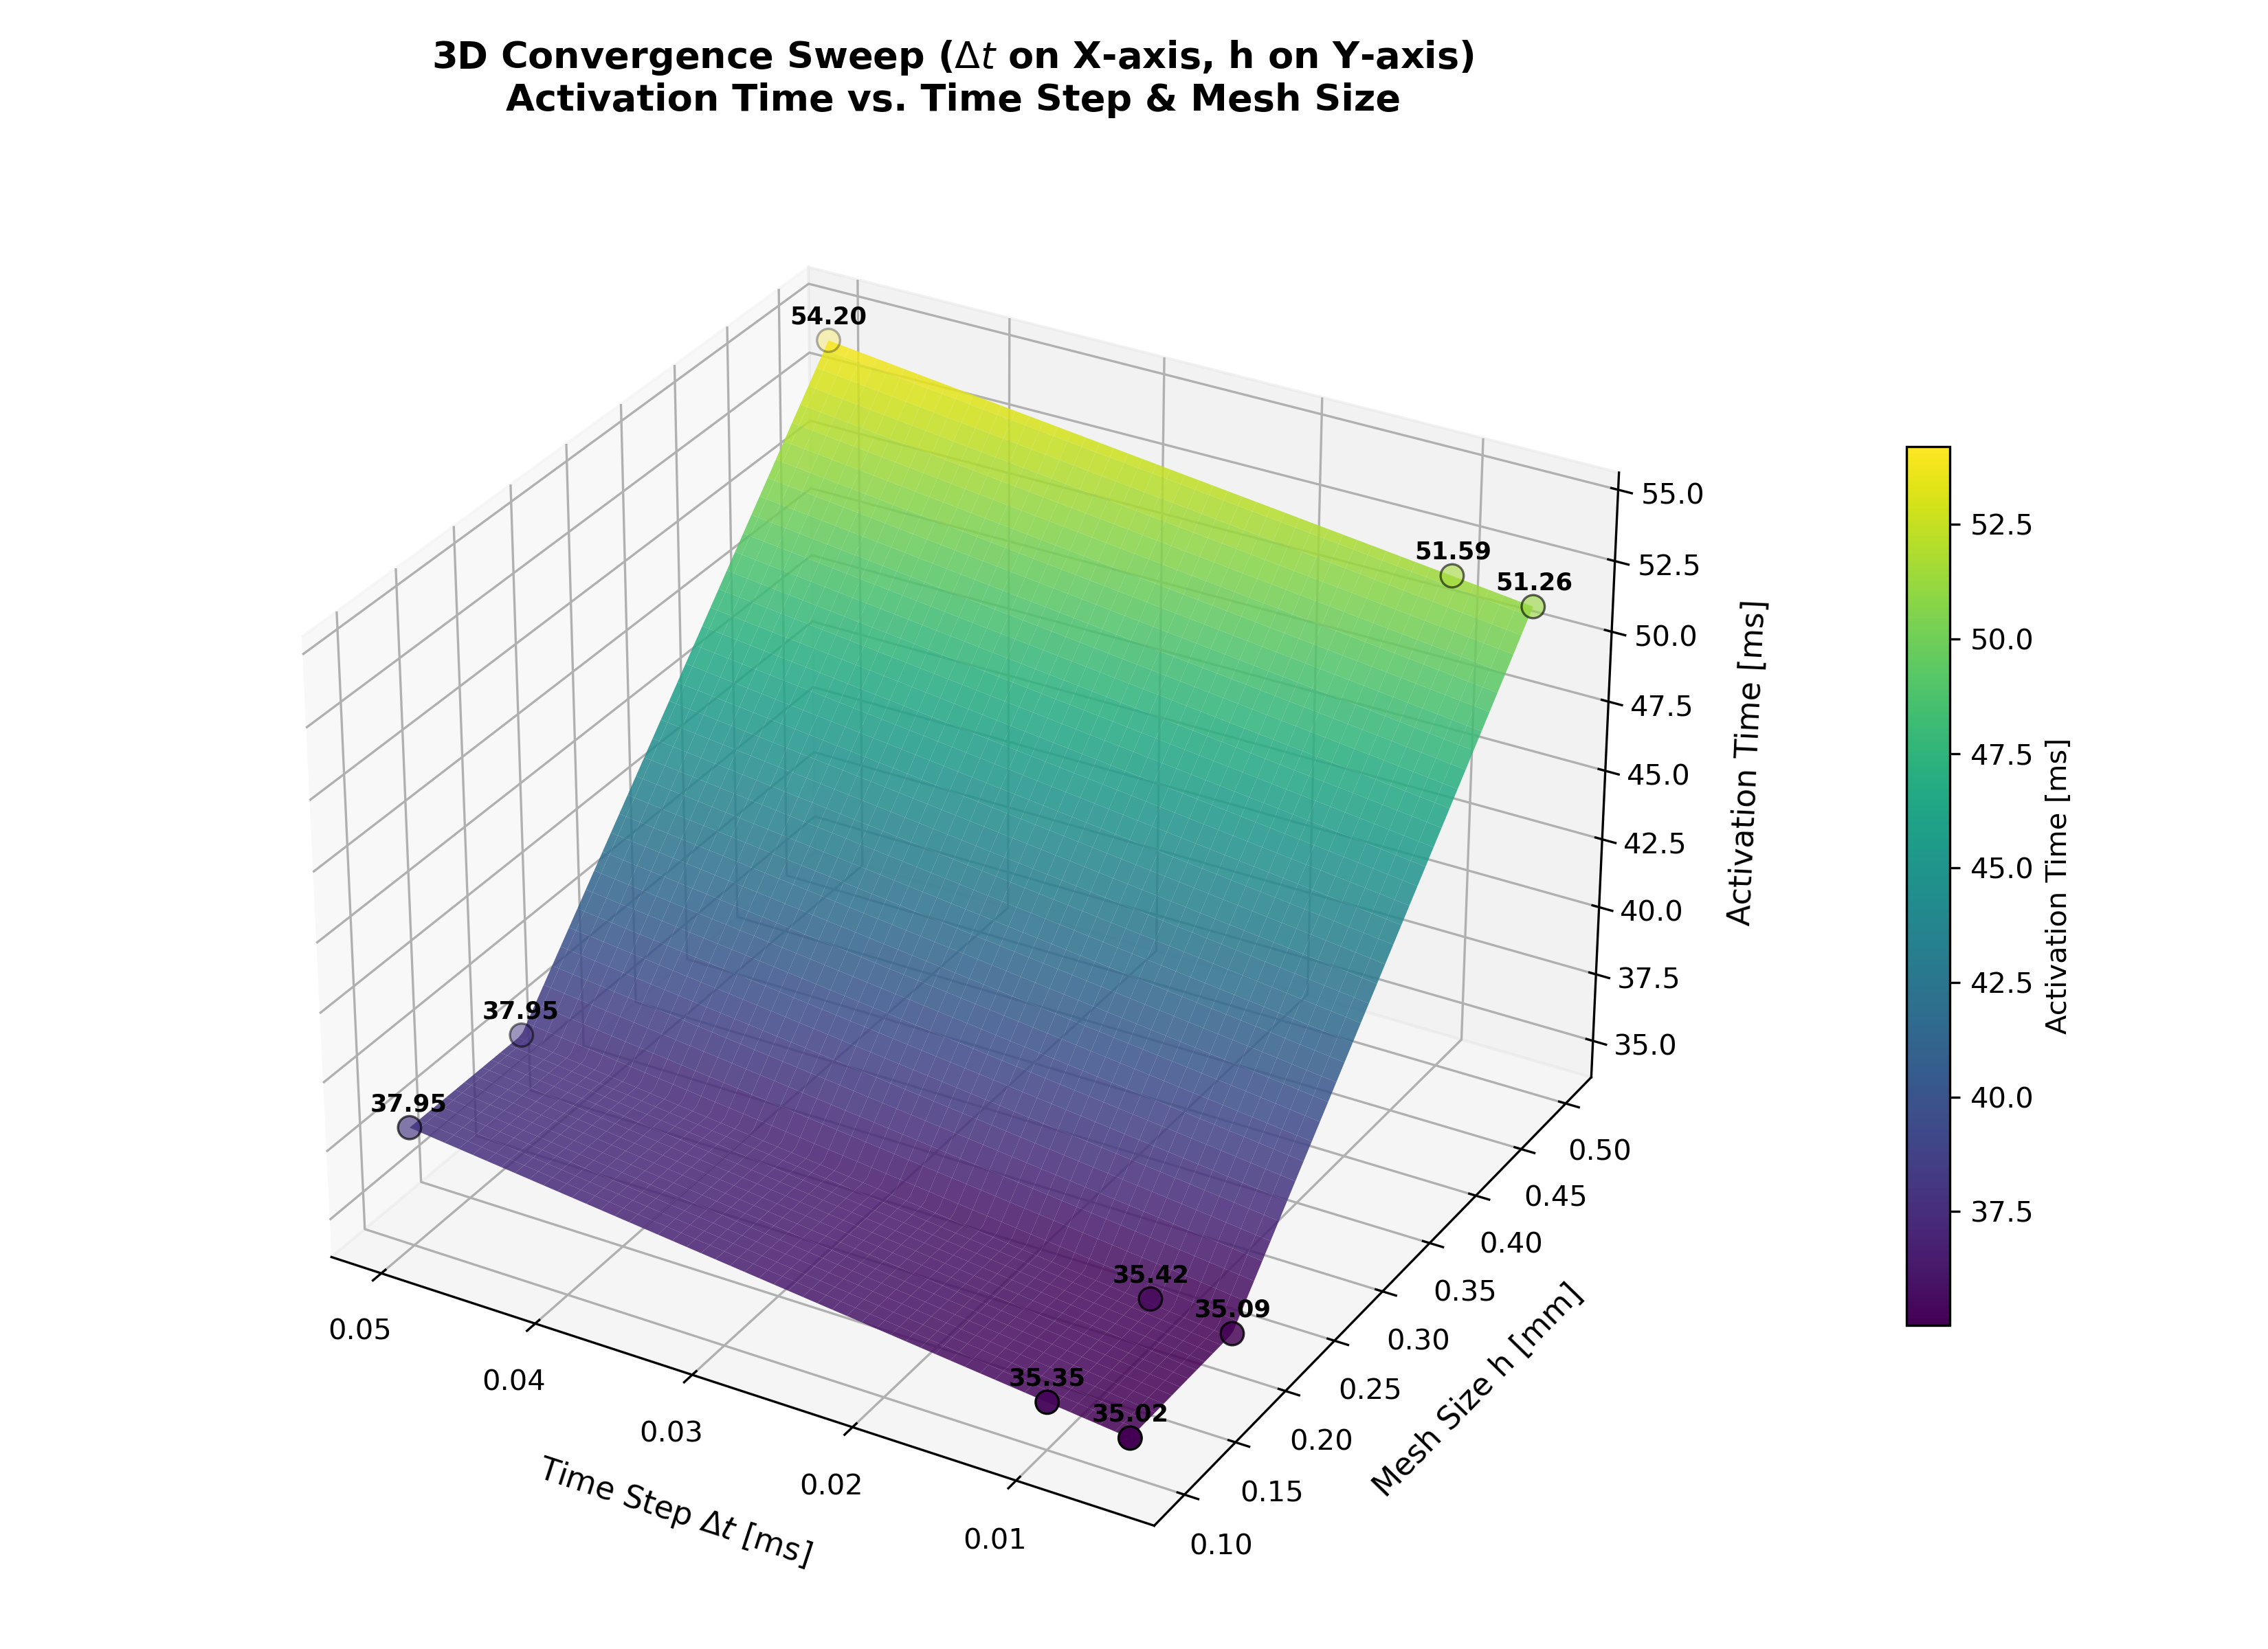
\includegraphics[width=0.8\textwidth]{beamerthemepolimi_img/convergence_activation_time_3d.png}
\end{center}
\end{frame}

\begin{frame}{Time Discretization Schemes Comparison}
\begin{itemize}
  \item $\theta=0$ (Forward Euler), $\theta=1$ (Backward Euler), $\theta=0.5$ (Crank-Nicolson);
  \item Curves nearly coincident at macroscopic scale;
  \item Minor discrepancies only in the terminal phase;
  \item Confirms $O(\Delta t)$ overall accuracy, independent of $\theta$.
\end{itemize}

\end{frame}

\begin{frame}{Time Discretization Schemes Comparison}
    \begin{center}
    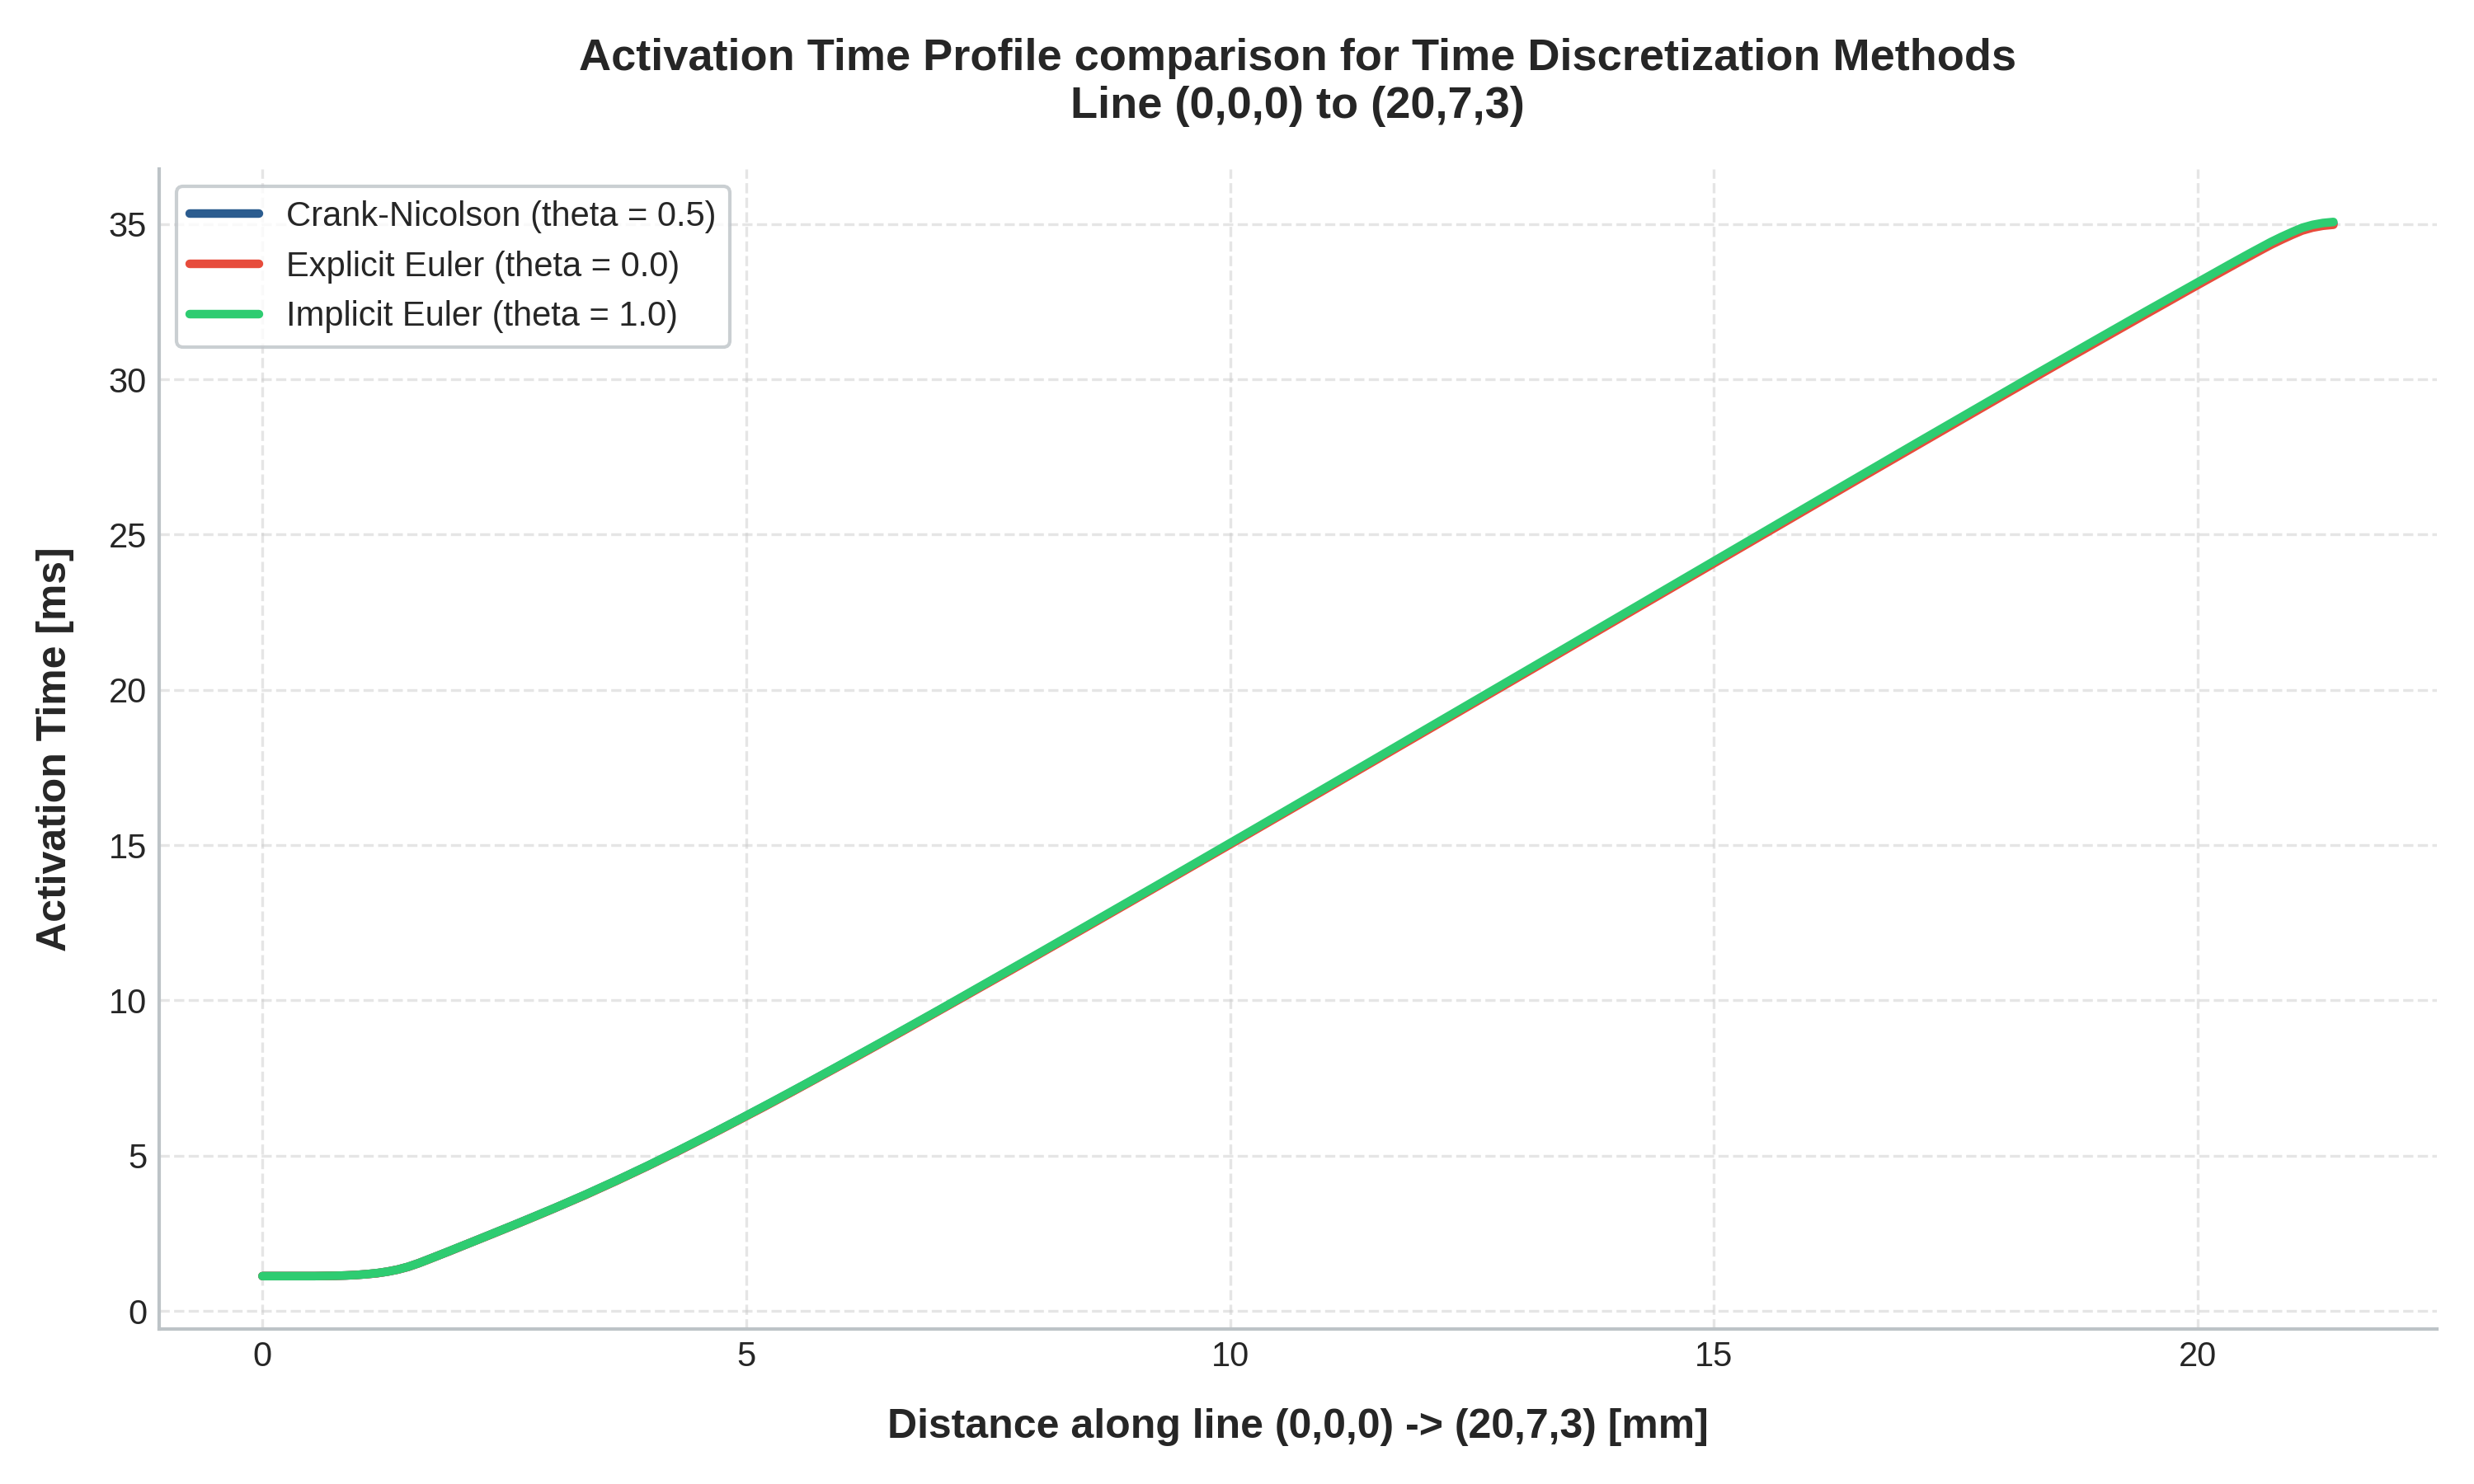
\includegraphics[width=0.9\textwidth]{beamerthemepolimi_img/euler_comparison_over_line.png}
\end{center}
\end{frame}
\begin{frame}{Time Discretization Schemes Comparison}
    \begin{center}
    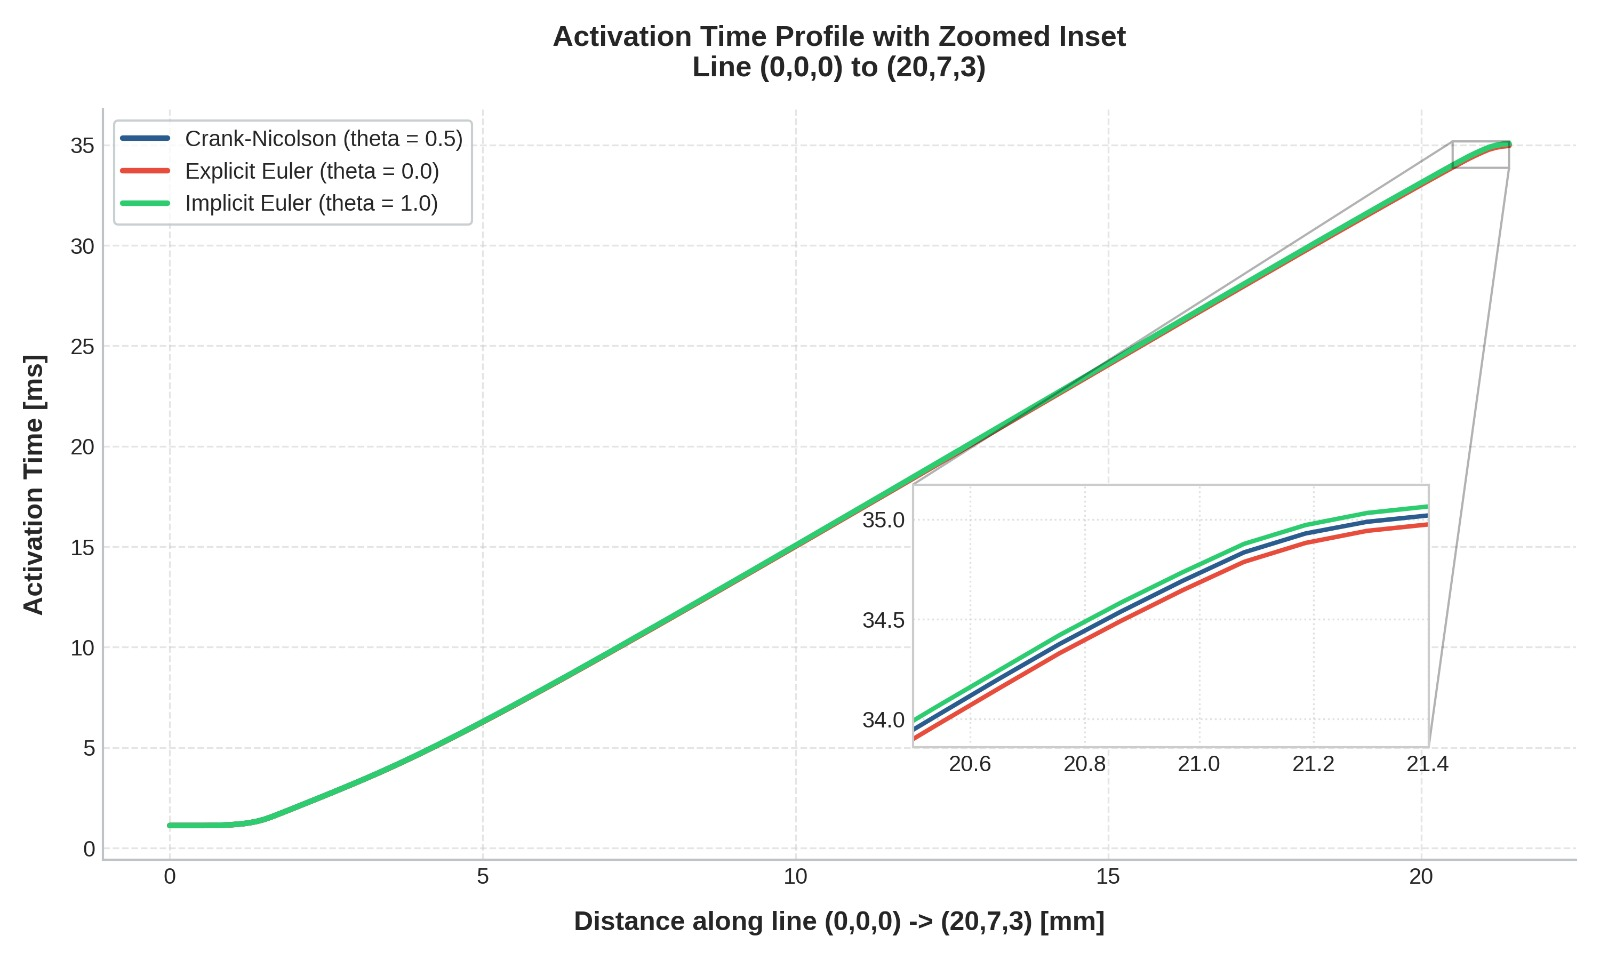
\includegraphics[width=0.9\textwidth]{beamerthemepolimi_img/theta_zoom_inset.jpeg}
\end{center}
\end{frame}
\begin{frame}{Linear Solvers and Preconditioners}
\begin{itemize}
  \item CG + ILU(0): best performance, $47.86$ min average;
  \item Increasing ILU fill-in: no practical benefit (avg. iterations $\approx 10.8$);
  \item SSOR: worse performance (higher arithmetic cost, more iterations);
  \item Direct solver: worst performance ($269.51$ min) due to severe fill-in
        on $442{,}401$ DoFs.
\end{itemize}

\end{frame}
\begin{frame}{Linear Solvers and Preconditioners}
    \begin{center}
    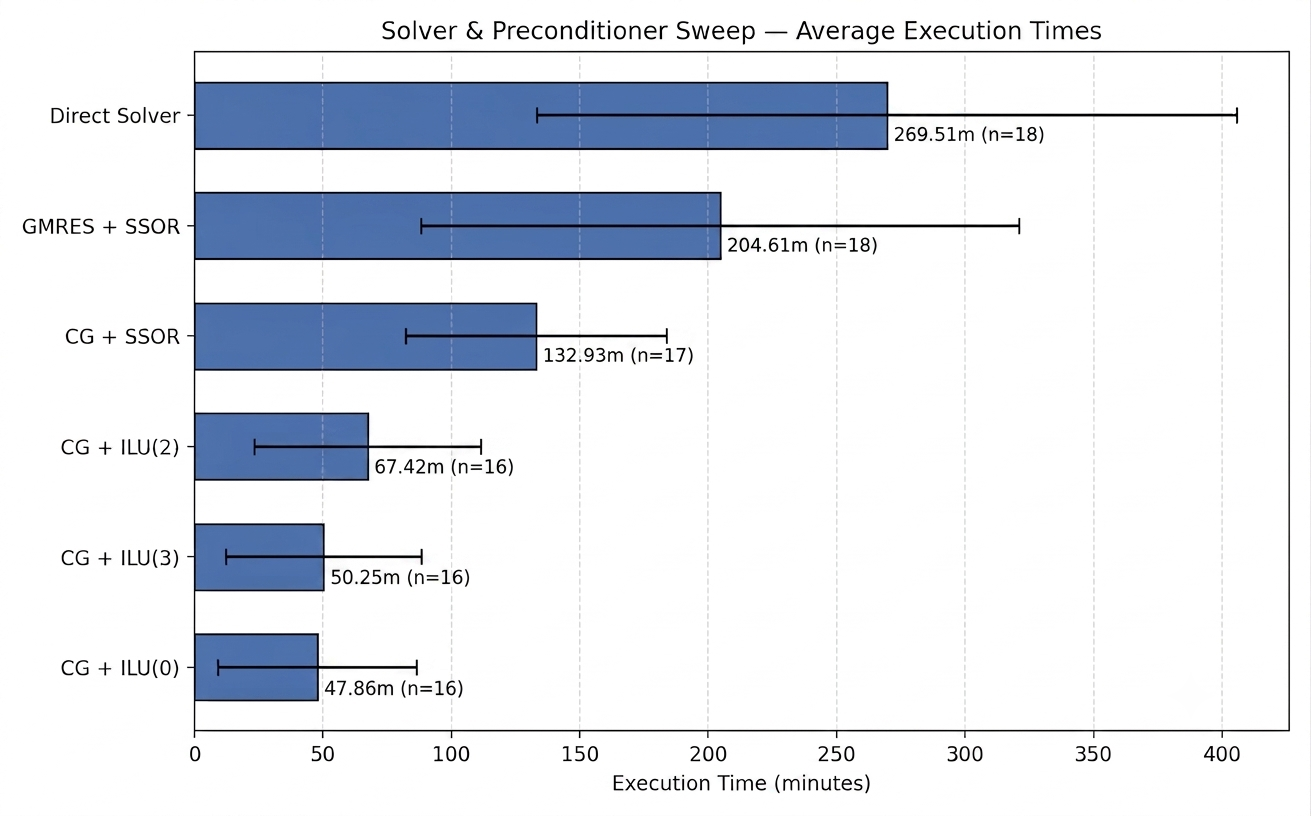
\includegraphics[width=0.9\textwidth]{beamerthemepolimi_img/solver_performance_avg.png}
\end{center}
\end{frame}

\begin{frame}{Linear Solvers and Preconditioners}
    \begin{center}
    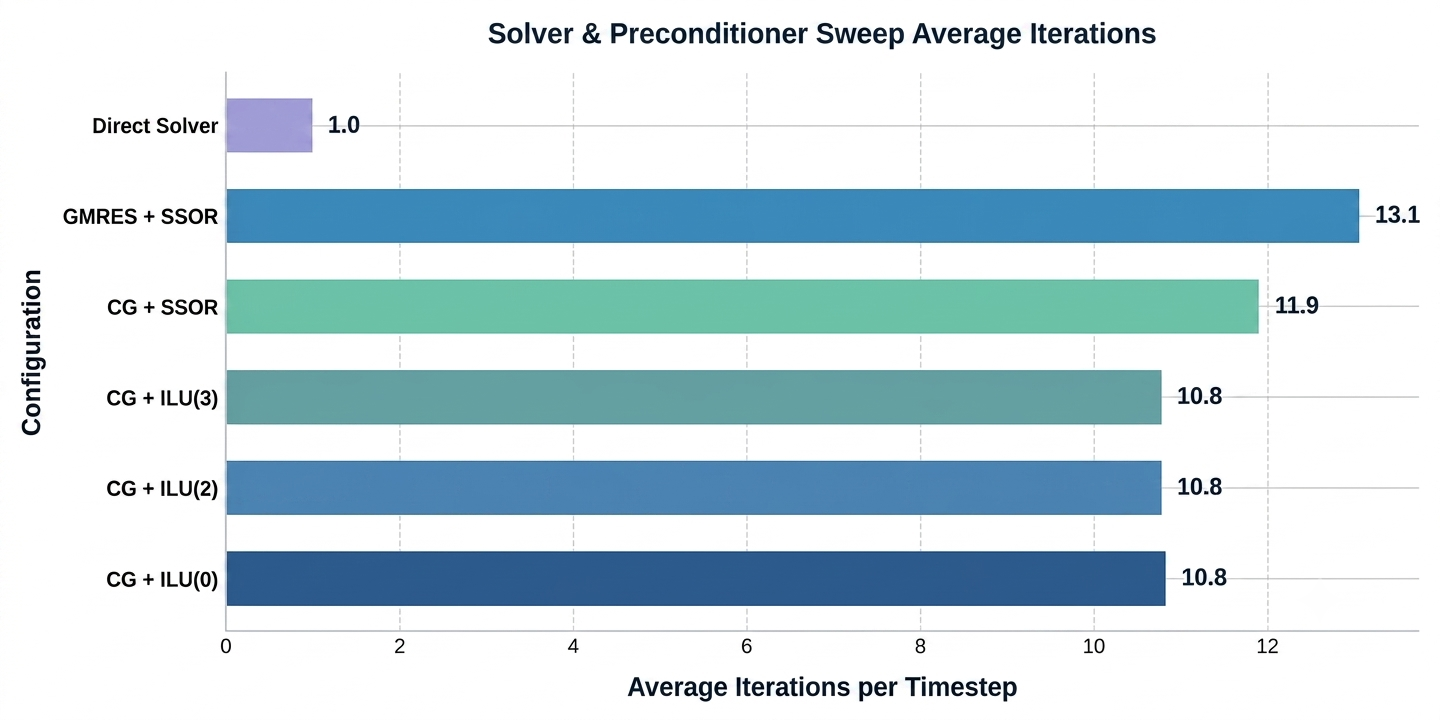
\includegraphics[width=0.8\textwidth]{beamerthemepolimi_img/solver_average_iterations .png}
\end{center}
\end{frame}

\begin{frame}{Simulation of Different Parameter Sets}

The simulations are performed using these five parameter sets:

\begin{itemize}
    \item \textbf{EPI}: Epicardial tissue
    \item \textbf{ENDO}: Endocardial tissue
    \item \textbf{M}: Midmyocardial tissue (M cells)
    \item \textbf{PB}: Parameter set reproducing the Priebe--Beuckelmann model
    \item \textbf{TNNP}: Parameter set reproducing the Ten Tusscher--Noble--Noble--Panfilov model
\end{itemize}

\end{frame}



% \begin{frame}{Simulation of different parameter sets}
% \begin{itemize}
%     \item 
% Among all ionic current components, Jfi
%     is the primary contributor to the activation time.
%     \item
%     \[
% J_{fi} = -w_1\cdot H(v-\theta_{w1})\cdot(v-\theta_{w1})\cdot\frac{(v_v-v)}{\tau_{fi}}
% \]
% \end{itemize}
% \textbf{Model} & $\tau_{fi}$ (ms) & $\theta_{w_1}$ & $v_u$ & \\
% \begin{tabular}{lcccc} 
% \hline
% M    & 0.078 & 0.30 & 1.61 & highest \\
% ENDO & 0.100 & 0.30 & 1.56 & high    \\
% EPI  & 0.110 & 0.30 & 1.55 & high    \\
% TNNP & 0.110 & 0.30 & 1.58 & medium  \\
% PB   & 0.105 & 0.35 & 1.45 & lowest  \\
% \hline
% \end{tabular}

% \end{frame}


\begin{frame}{Simulation of different parameter sets}

\begin{figure}
\centering

% Riga superiore
\begin{minipage}{0.25\textwidth}
    \centering
    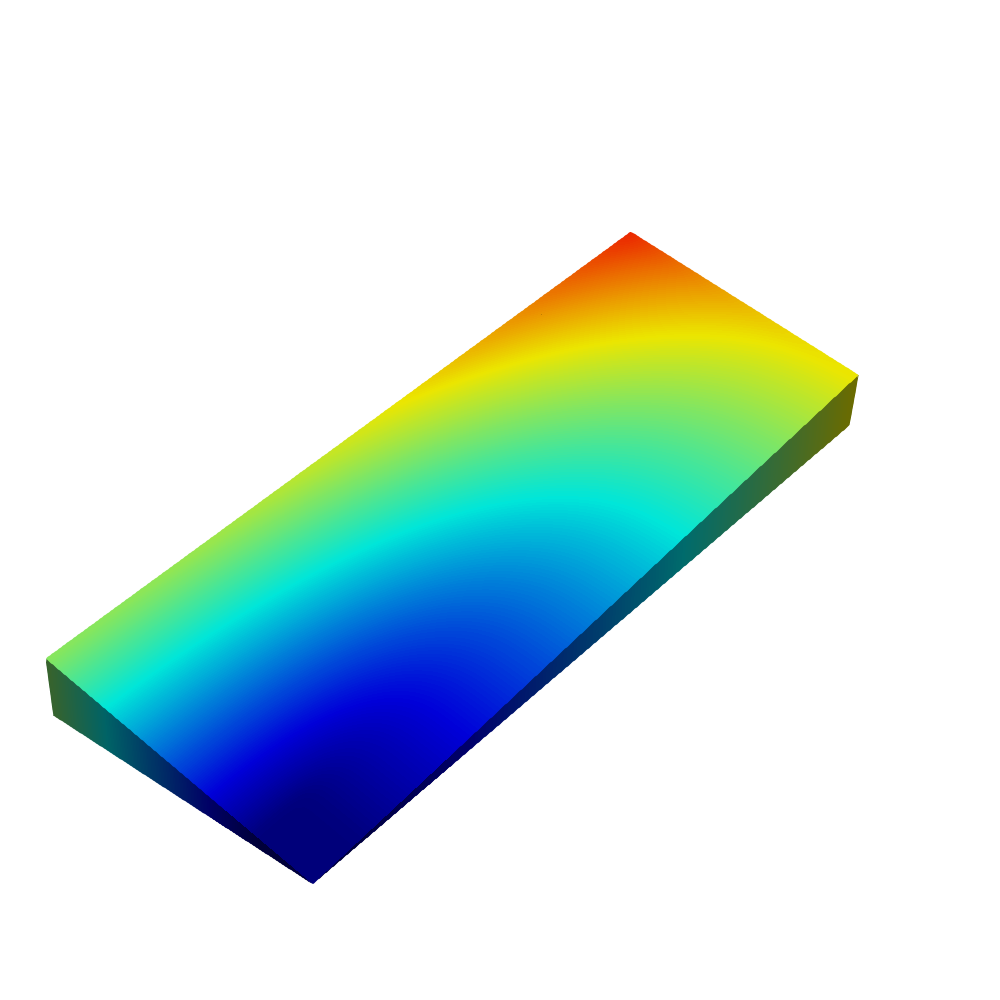
\includegraphics[width=\textwidth]{beamerthemepolimi_img/EPI_activation_time_0_clip.png}
    \scriptsize EPI
\end{minipage}
\hfill
\begin{minipage}{0.25\textwidth}
    \centering
    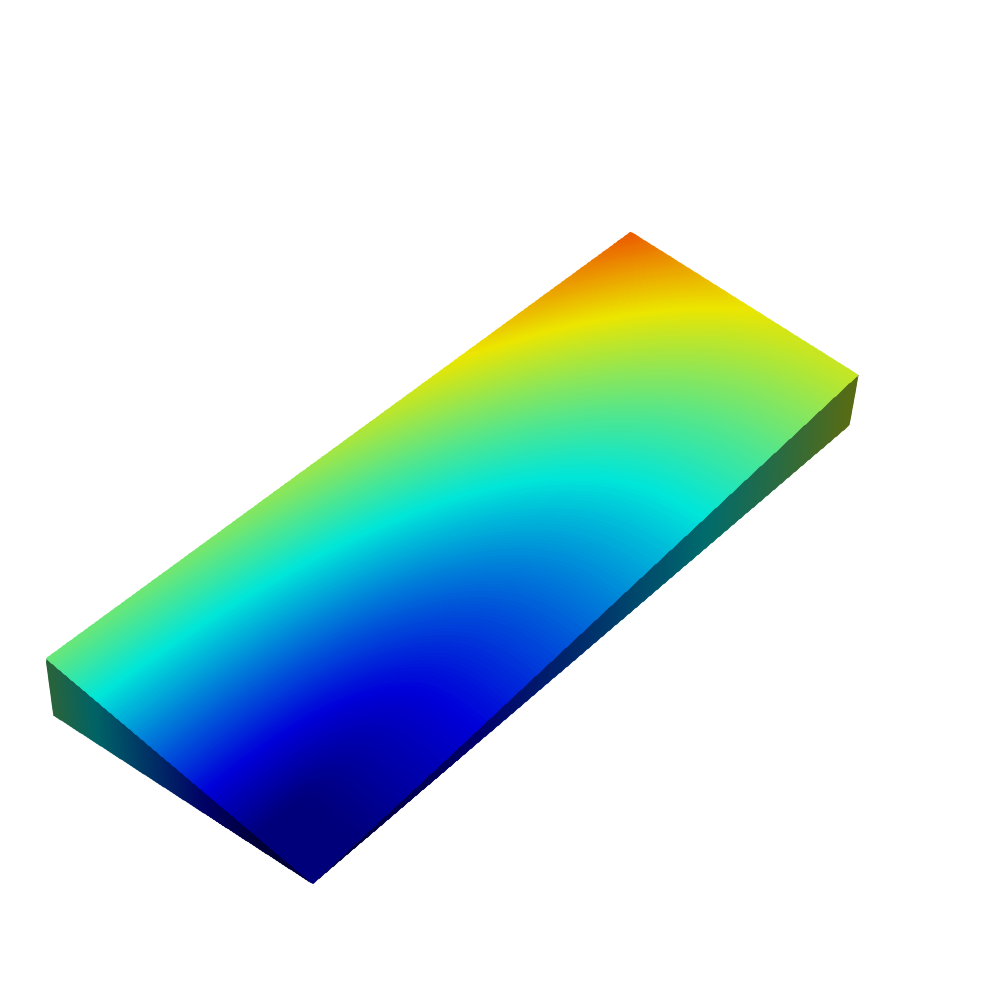
\includegraphics[width=\textwidth]{beamerthemepolimi_img/ENDO_activation_time_0_clip.png}
    \scriptsize ENDO
\end{minipage}
\hfill
\begin{minipage}{0.25\textwidth}
    \centering
    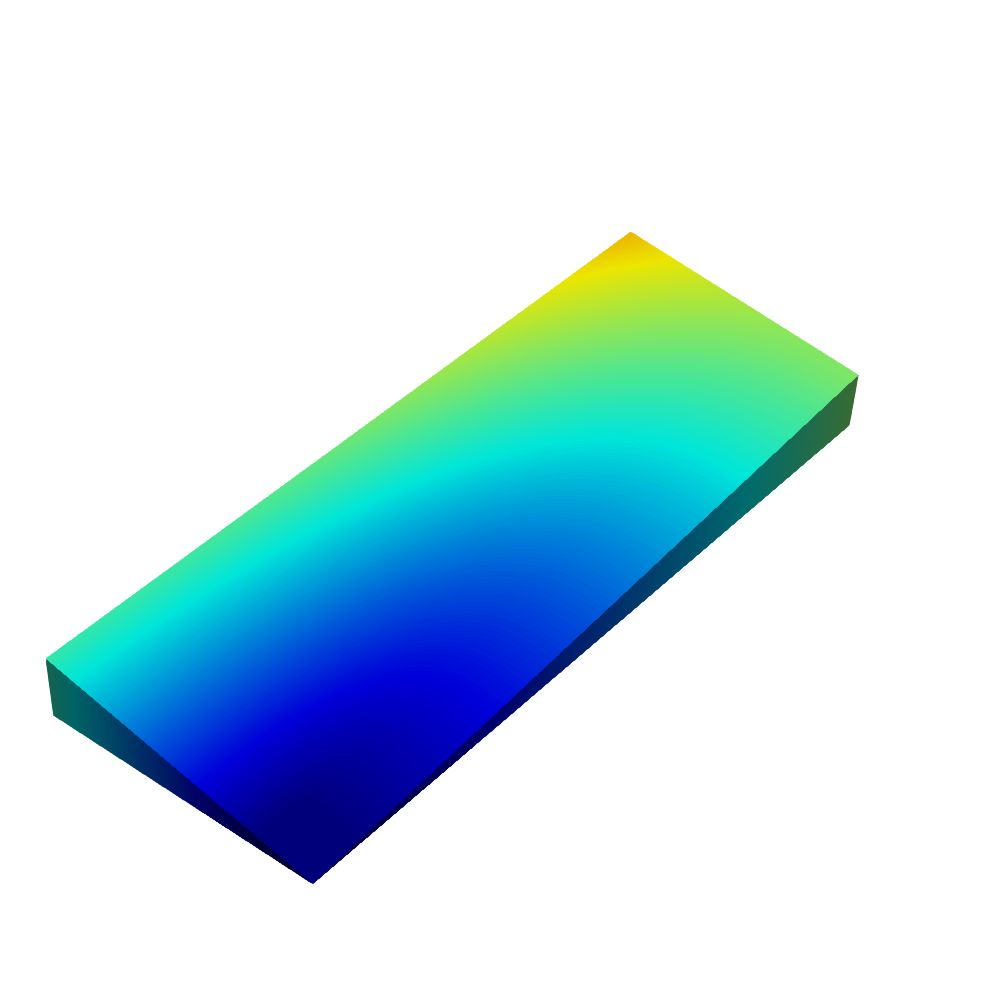
\includegraphics[width=\textwidth]{beamerthemepolimi_img/M_activation_time_0_clip.png}
    \scriptsize M
\end{minipage}
% Riga inferiore
\begin{minipage}{0.25\textwidth}
    \centering
    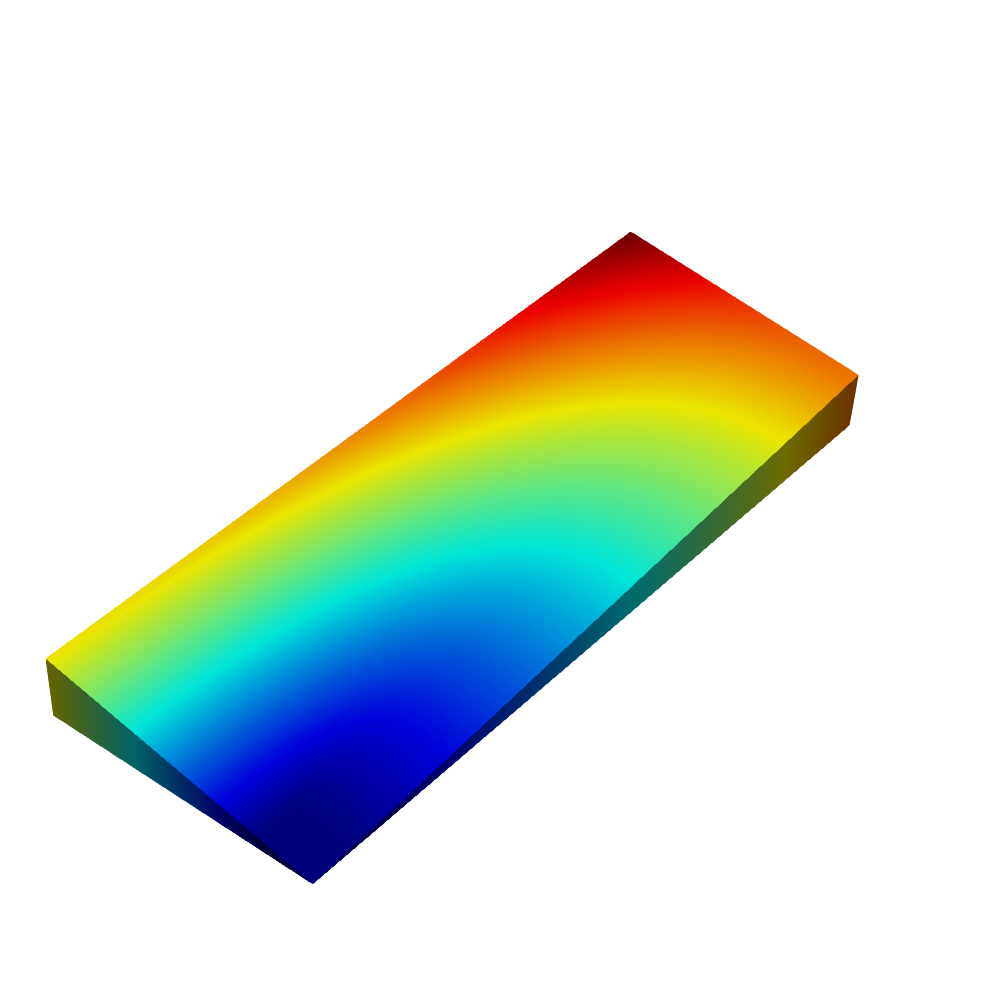
\includegraphics[width=\textwidth]{beamerthemepolimi_img/PB_activation_time_0_clip.png}
    \scriptsize PB
\end{minipage}
\hfill
\begin{minipage}{0.25\textwidth}
    \centering
    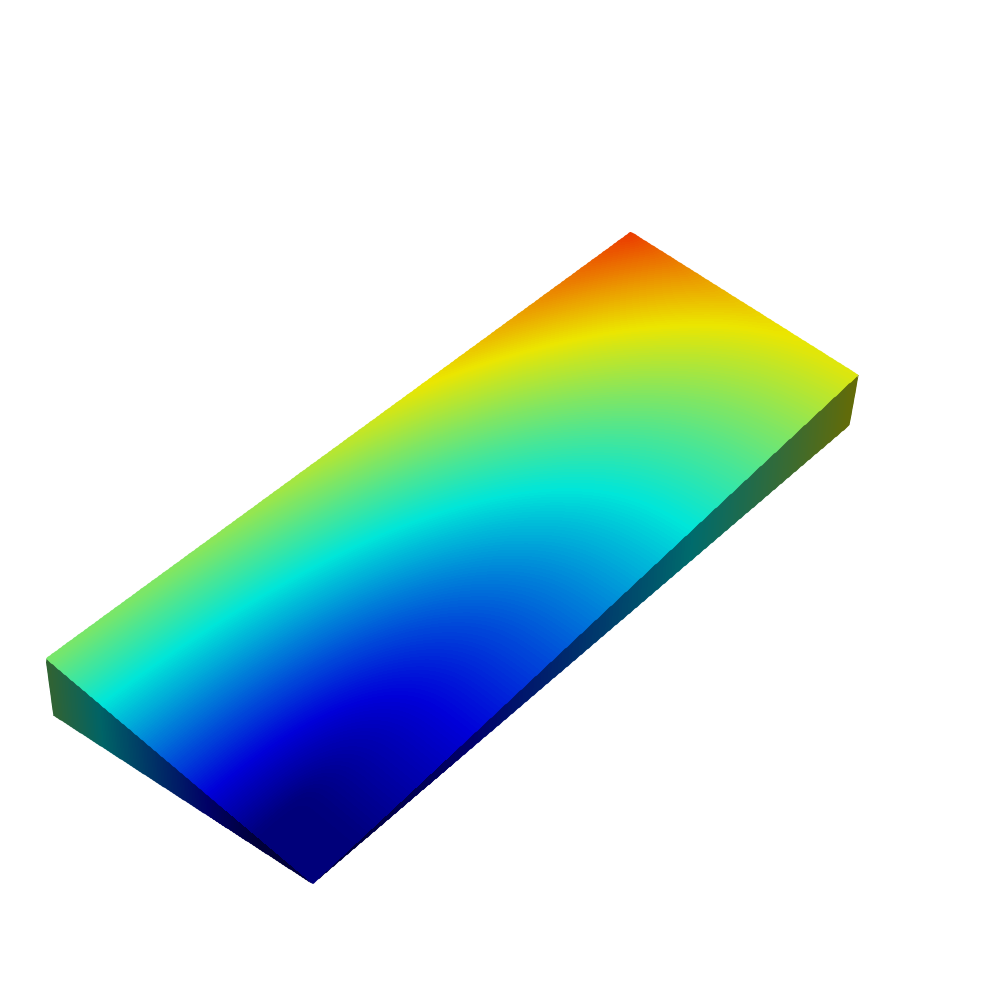
\includegraphics[width=\textwidth]{beamerthemepolimi_img/TNNP_activation_time_0_clip.png}
    \scriptsize TNNP
\end{minipage}
\hfill
\begin{minipage}{0.10\textwidth}
    \centering
    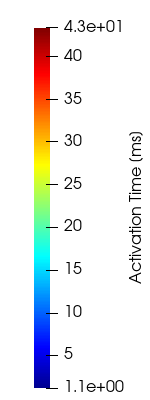
\includegraphics[width=\textwidth]{beamerthemepolimi_img/colorbar_legend.png}
\end{minipage}

\end{figure}

\end{frame}
\begin{frame}{Simulation of different parameter sets}
    \begin{center}
    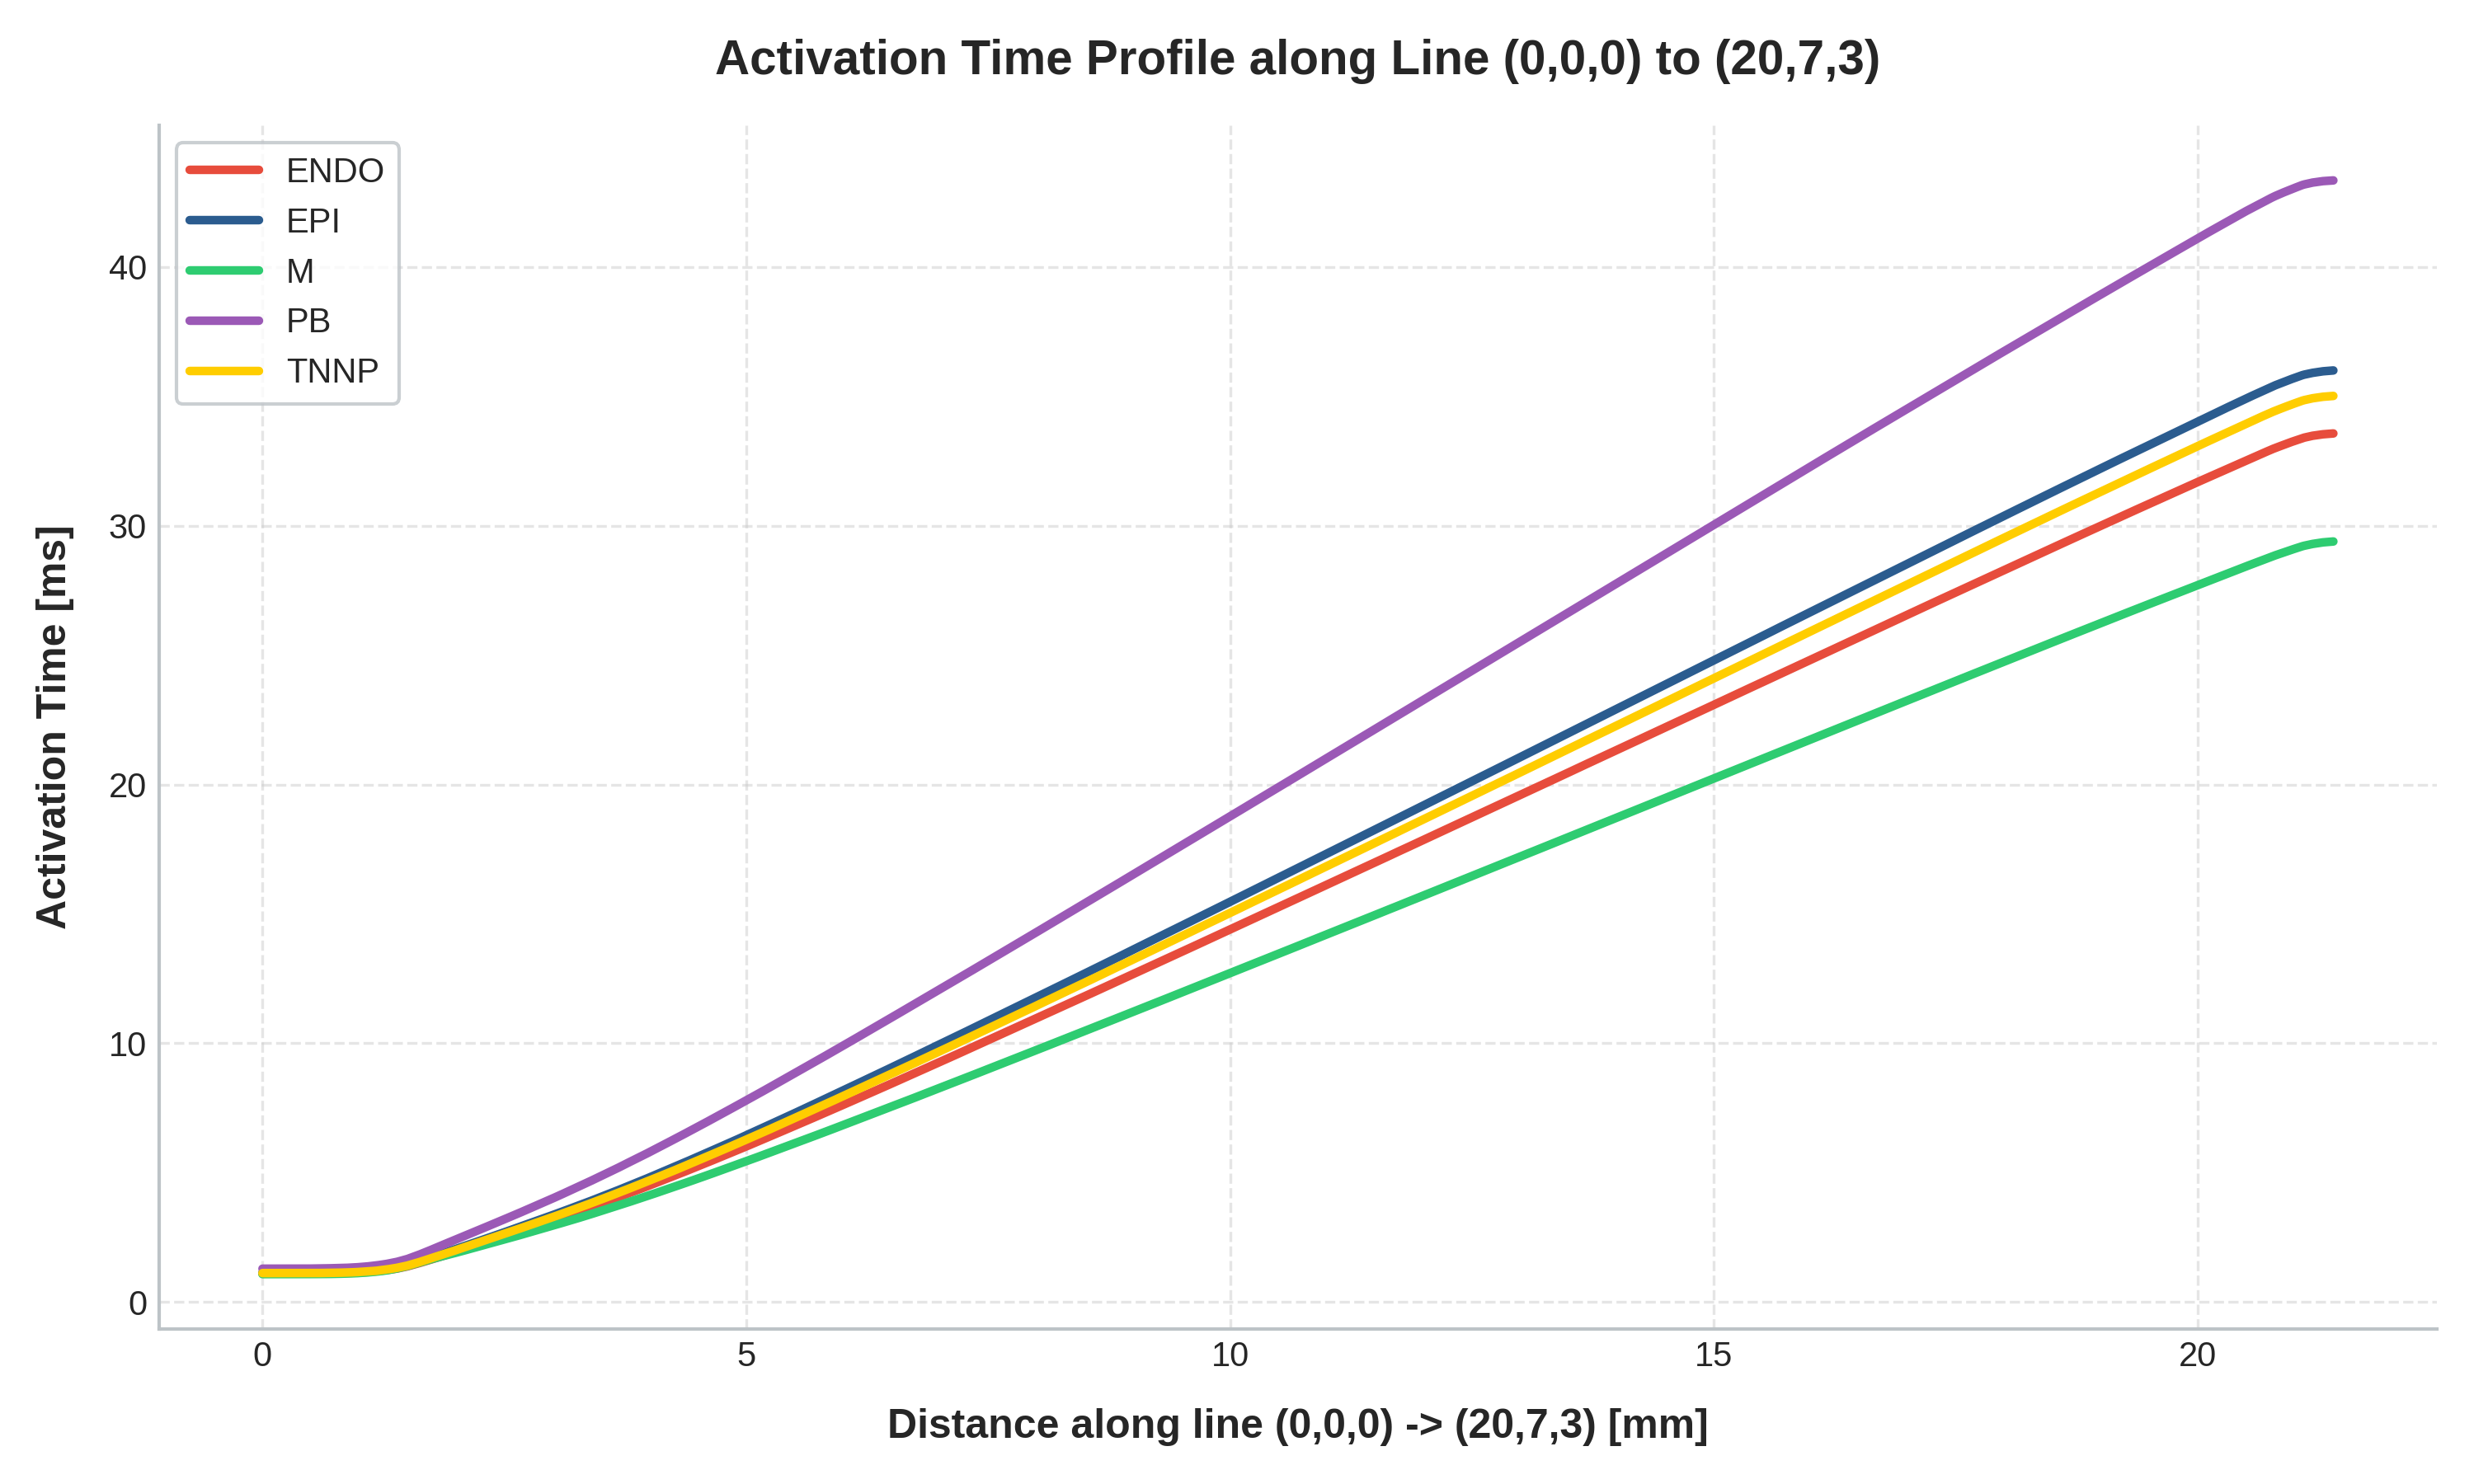
\includegraphics[width=0.8\textwidth]{beamerthemepolimi_img/activation_time_over_line.png}
\end{center}
\end{frame}
\begin{frame}{Simulation of different parameter sets}
    \begin{center}
    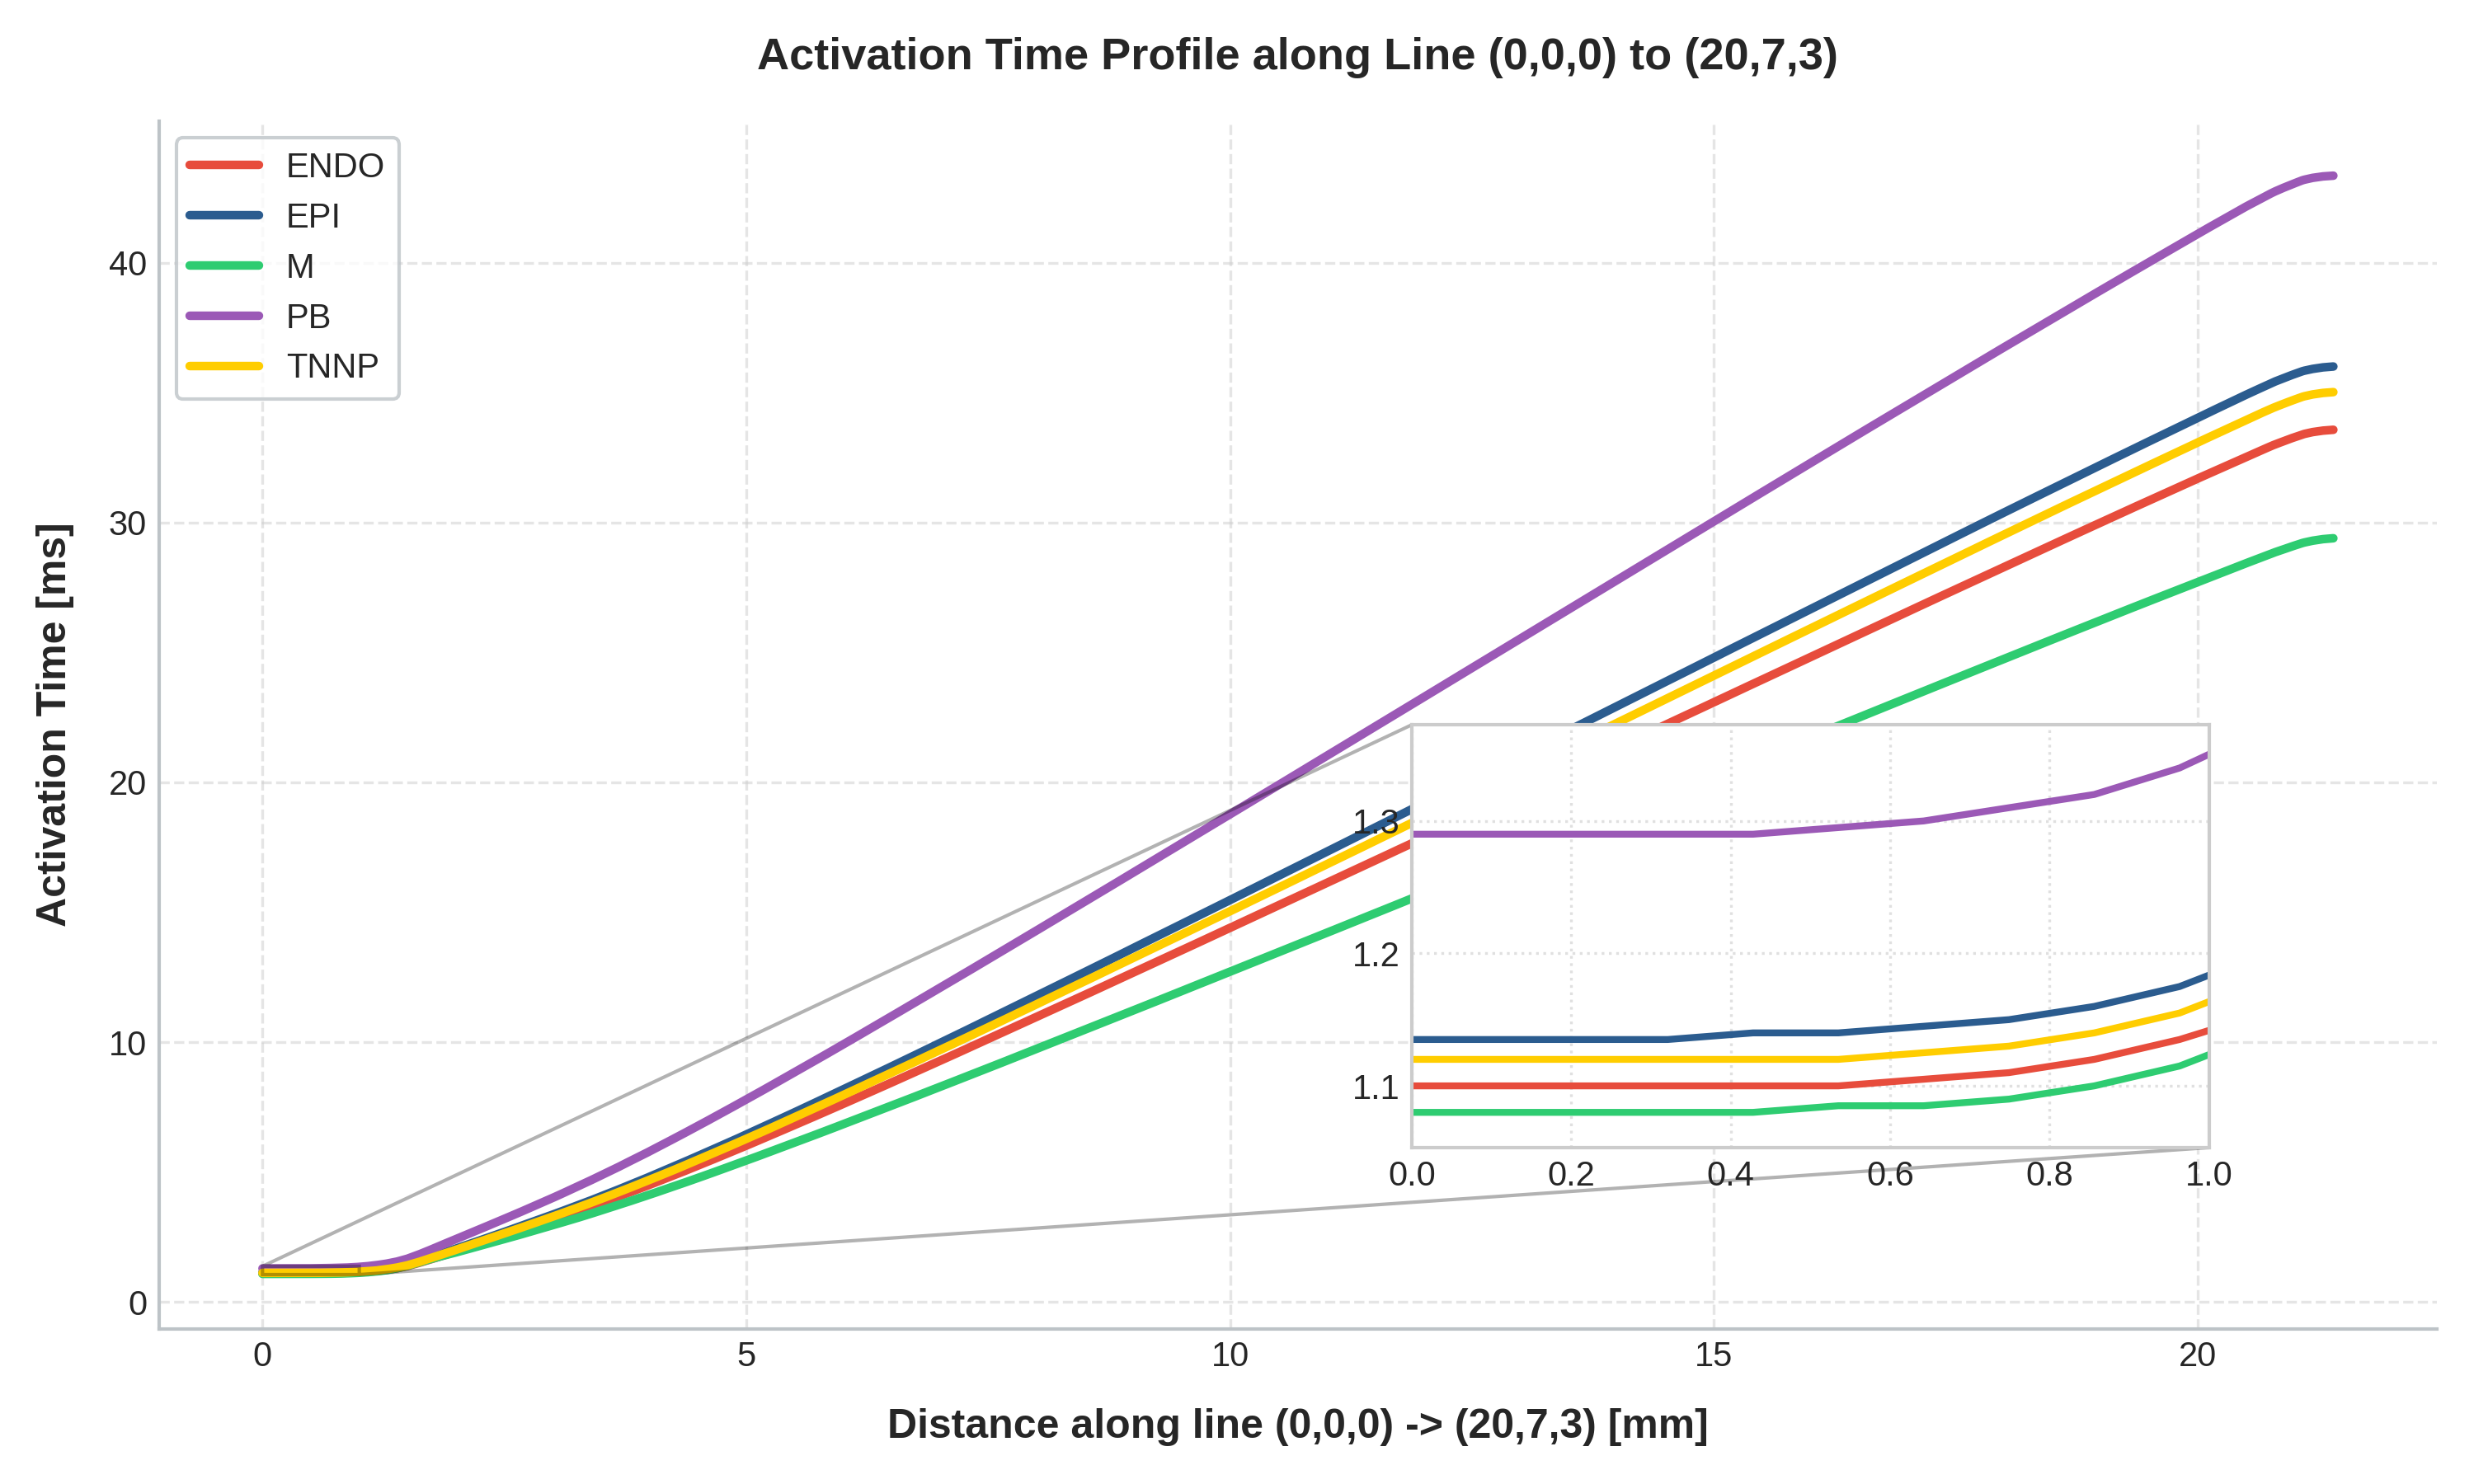
\includegraphics[width=0.8\textwidth]{beamerthemepolimi_img/activation_time_over_line_combined.png}
\end{center}
\end{frame}
\begin{frame}{Simulation of different parameter sets}
\begin{itemize}
    \item 
Among all ionic current components, Jfi
    is the primary contributor to the activation time.
    \item
    \[
J_{fi} = -w_1\cdot H(v-\theta_{w1})\cdot(v-\theta_{w1})\cdot\frac{(v_u-v)}{\tau_{fi}}
\]
\end{itemize}
\begin{table}[h]
\centering
\begin{tabular}{lcccc}
\hline
\textbf{Model} & \boldmath$\tau_{fi}$ & \boldmath$\theta_{w1}$ & \boldmath$v_u$ & \textbf{Prop. speed}  \\
\hline
M    & 0.078 & 0.30 & 1.61 & High \\
ENDO & 0.100 & 0.30 & 1.56 & Medium \\
EPI  & 0.110 & 0.30 & 1.55 & Medium \\
TNNP & 0.110 & 0.30 & 1.58 & Medium \\
PB   & 0.105 & 0.35 & 1.45 & Low \\
\hline
\end{tabular}
\end{table}

\end{frame}
% \begin{frame}{Scalability}
% \begin{itemize}
%   \item Average execution time: $234.59$ min (1 proc.) $\to$ $83.73$ min (16 proc.);
%   \item Practical limit: $\le 16$ MPI processes, or two-level/Schwarz preconditioners.
%   \item Performance degrades when scaling from 16 to 32 MPI, then it slightly improves from 32 to 56 MPI
%   \item Every execution is affected by cluster noise
     
% \end{itemize}
% \end{frame}


\begin{frame}{Scalability}
    \begin{center}
    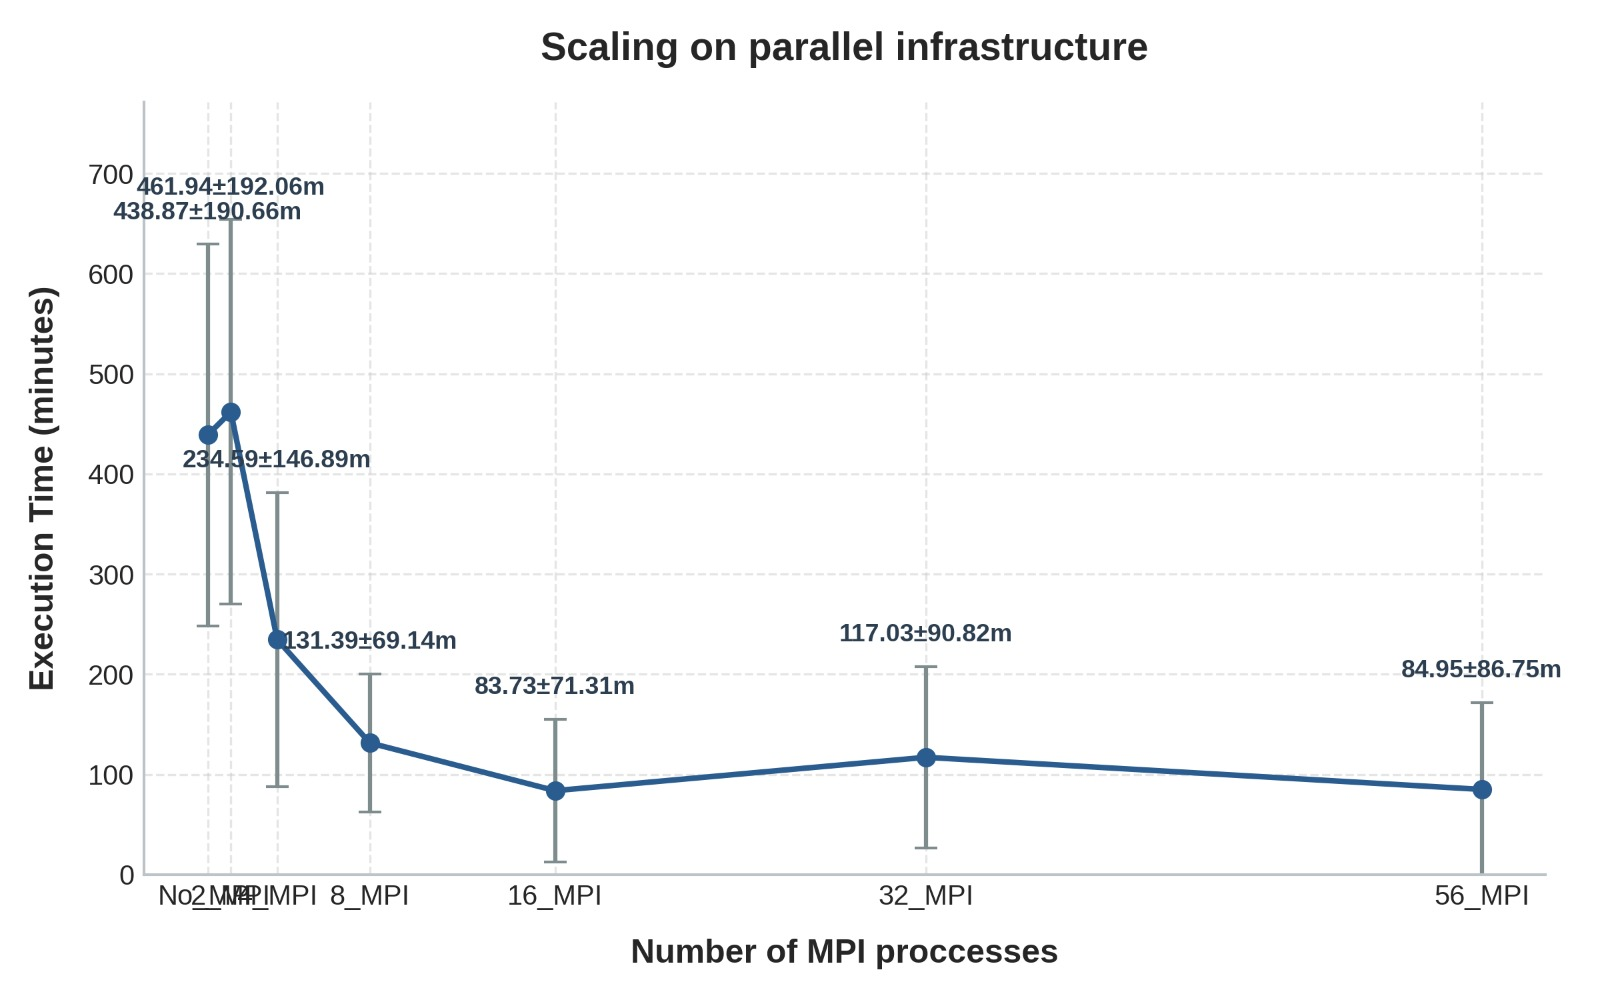
\includegraphics[width=0.8\textwidth]{beamerthemepolimi_img/scalability.jpeg}
\end{center}
\end{frame}
\begin{frame}{Scalability}
    \begin{center}
    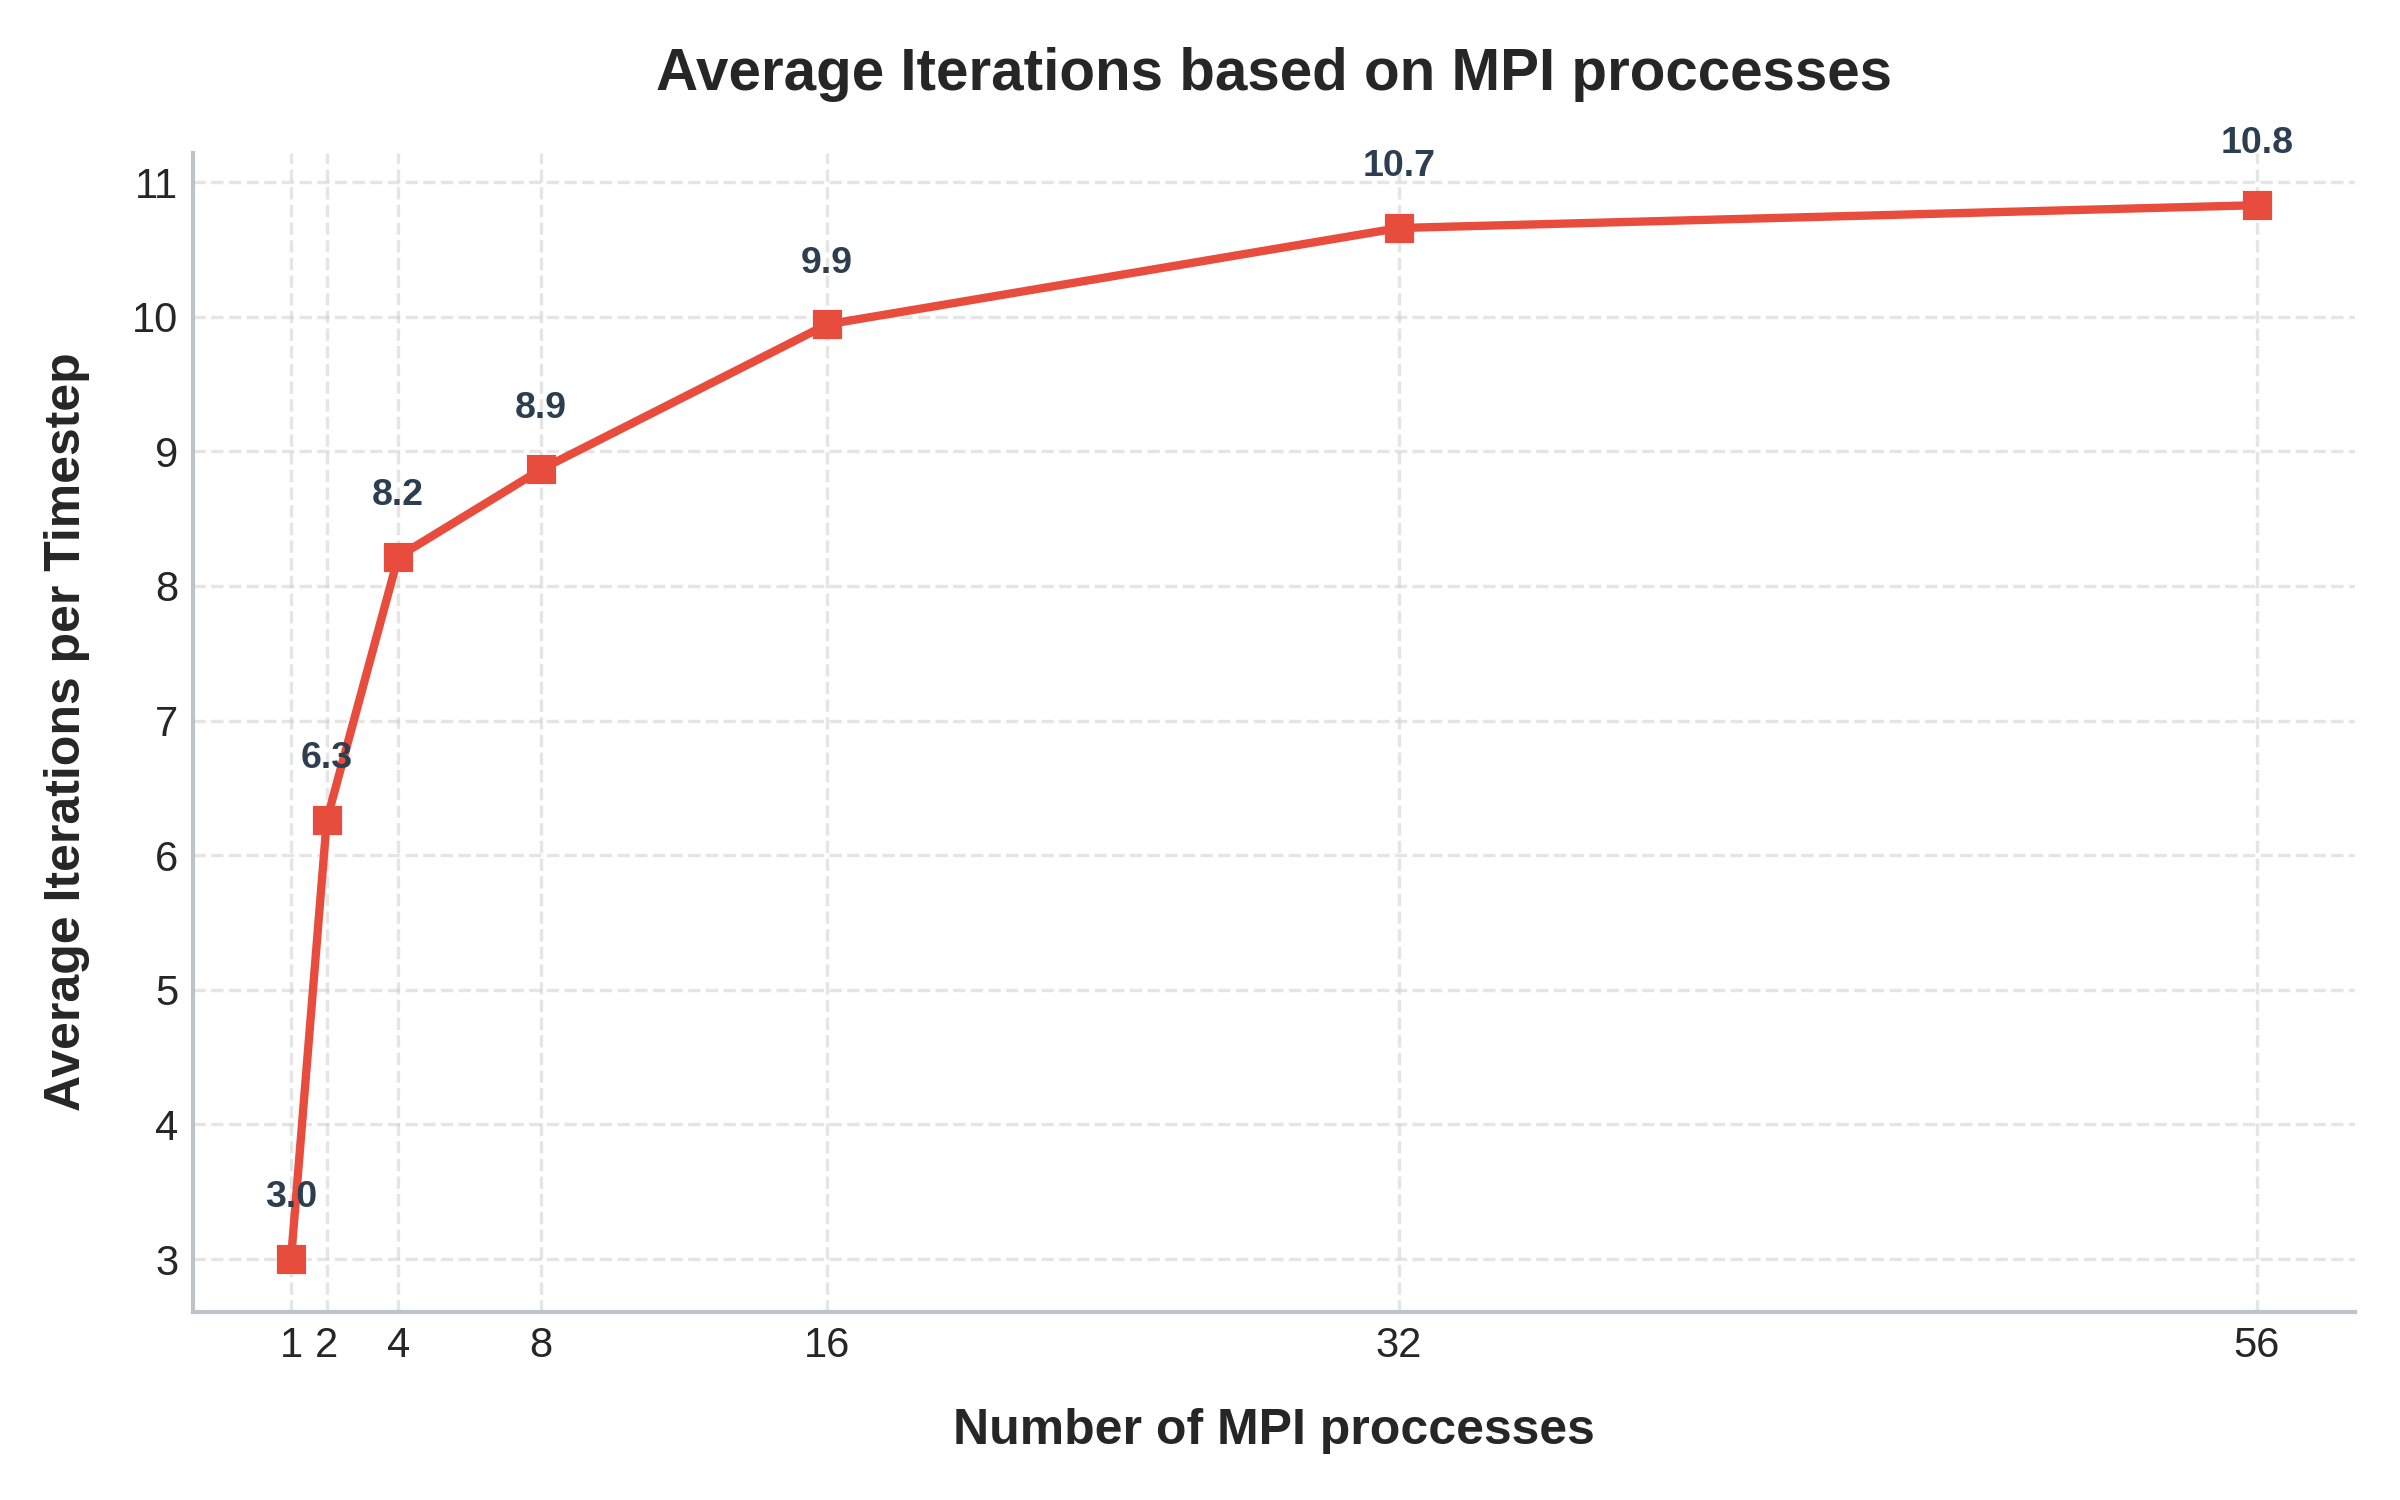
\includegraphics[width=0.8\textwidth]{beamerthemepolimi_img/scalability_average_iterations.png}
\end{center}
\end{frame}
\begin{frame}{Scalability}
\begin{itemize}
  \item Average execution time: $234.59$ min (1 proc.) $\to$ $83.73$ min (16 proc.);
  \item Best performance achieved with $16$ MPI processes
  \item Performance degrades when scaling from 16 to 32 MPI, then it slightly improves from 32 to 56 MPI
  \item Every execution is affected by cluster noise
     
\end{itemize}
\end{frame}
% ============================================================
\section{}
% ============================================================

\begin{frame}{Conclusions}
\begin{itemize}
  \item Effective trade-off between physiological accuracy and computational cost;
  \item IMEX $\theta$-scheme + explicit gating update: avoids nonlinear coupled solves;
  \item CG + ILU(0): most efficient linear solver configuration;
  \item Model flexibility confirmed across 5 parameter sets;
  \item Future work: quantitative validation vs.\ Bueno-Orovio and
        Niederer et al.\ benchmark; more robust preconditioners for strong scaling.
\end{itemize}
\end{frame}

\begin{frame}{Bibliography}
\begin{itemize}
\item A. Bueno-Orovio, E. M. Cherry, and F. H. Fenton. Minimal model for human
ventricular action potentials in tissue. Journal of Theoretical Biology, 253(3):544–
560, 2008.
\item S. A. Niederer, E. Kerfoot, A. P. Benson, M. O. Bernabeu, O. Bernus, C. Bradley, E. M. Cherry, R. Clayton, F. H. Fenton, A. Garny, et al. Verification of cardiac
tissue electrophysiology simulators using an N-version benchmark. Philosophical
Transactions of the Royal Society A: Mathematical, Physical and Engineering Sciences,
369(1954):4331–4351, 2011.
\end{itemize}

\end{frame}

\begin{frame}
    \centering
    \vfill

    {\Huge Thank you for your attention!}

    \vfill
\end{frame}

\end{document}